\documentclass[11pt,a4paper]{report}

\usepackage{hyperref}
\usepackage{caption}
\usepackage{amsfonts}
\usepackage{cite}
\usepackage{graphicx}
\usepackage{verbatim}
\usepackage{subfigure}
\graphicspath{ {images/} }

\author{Catherine Vlasov}
\title{Optimizing Learning Parameters Used by Reinforcement Learning Algorithms}
\date{23 April 2018}

\newcommand{\argmax}{\mathop{\mathrm{arg\,max}}}

\begin{document}

\makeatletter
	\begin{titlepage}
		\vspace*{\fill}
		\begin{center}
			{\huge \bfseries \@title }
			\\[4ex]
			{\LARGE  \@author}
			\\[2ex]
			{\large \@date}
			\\[50ex]
			
\includegraphics[width=30mm]{oxlogo.png}
		\end{center}
		\vspace*{\fill}
	\end{titlepage}
\makeatother


%-----------------------
\begin{abstract}
This is my abstract
\end{abstract}


%-----------------------
\tableofcontents


%-----------------------
\chapter{Introduction}

Over the last few decades, reinforcement learning has seen a large increase in popularity. It amazes the world again and again, whether playing Go \cite{go}, Backgammon \cite{backgammon}, or Atari \cite{atari} games, and its potential continues to grow. These successes were not lucky, but rather they were a product of studying the nature, size, and complexity of each task, choosing the algorithm best suited to it, and then setting up the algorithm appropriately. The last of these steps is crucial to the success of reinforcement learning for a particular task and must be done carefully. Thus, this project aims to elucidate how to set up a reinforcement learning algorithm by tuning its parameters, specifically for a particular class of algorithms called Monte Carlo algorithms.


\section{Goals}

The specific Monte Carlo algorithm this project implements and investigates is called an ``on-policy $\varepsilon$-soft Monte Carlo control algorithm''. Section \ref{sec:Terminology} explains the basics of reinforcement learning as well as terminology used throughout this report, such as ``on-policy'' and ``$\varepsilon$-soft''. As the name suggests, the algorithm uses a parameter $\varepsilon$ to guide its learning. Effectively, it determines the balance between exploitation (choosing actions that are best, according to what it currently knows) and exploration (trying new actions). Thus, the chosen value of $\varepsilon$ can have a large effect on an agent's learning rate and therefore success at a particular task.

The on-policy $\varepsilon$-soft Monte Carlo control algorithm is not the primary subject of many research papers since it is simple, relative to other popular reinforcement learning techniques. Consequently, there is a lack of guidance on how to apply the algorithm to real tasks and achieve the greatest success given constraints such as computing power and time.

The simplicity of the algorithm, however, facilitates an interesting analysis of the effect of the value of $\varepsilon$ on the algorithm's success rate. The overarching goal of this project is to develop a general technique for tailoring the algorithm to a particular reinforcement learning task, which can then be extended to other reinforcement learning algorithms with parameters that need to configured.

This project tackles a number of questions:

\begin{itemize}
	\item Are there ``optimal'' values of $\varepsilon$ that maximise the algorithm's performance?
	\item How quickly does the algorithm's policy converge? Does it converge to the theoretical optimal policy?
    \item How does the Monte Carlo with Exploring Starts algorithm (Monte Carlo ES \cite{rl-book}) affect the convergence rate of the policy?
	\item When playing games where states have axes of symmetry, how does the agent's 
performance and learning change when symmetry is eliminated?
	\item How does the performance of the algorithm differ for different games?
\end{itemize}

Three games were selected for this project: Tic-Tac-Toe, Chung Toi, and Nim. They are discussed in further detail in Section \ref{sec:DesignImpl}. They form an interesting mix since some have relatively long episodes, others can be used to investigate symmetry, and some with a similar state space can be compared against each other. Thus, it was possible to answer all of the above questions and derive some interesting results.



%-----------------------
\chapter{Background}

This section provides an overview of the theory behind reinforcement learning and the particular algorithm studied in this project.

\section{Reinforcement Learning}
\label{sec:RL}

Reinforcement learning (RL) is an area of machine learning in which an agent interacts with an environment by choosing actions, with the goal of maximizing the cumulative reward it receives for these actions.

The beauty of RL is that the agent is not given any information about \emph{how} to solve a problem, but rather it has to find out what works and what does not through trial-and-error. For this reason, RL is different from supervised learning because the agent is not provided with any input-output pairs to learn from. Instead, it learns and improves purely based on its own experiences.

RL is now described more formally. An \emph{agent} is a learner and the \emph{environment} is everything outside the agent, namely the thing that the agent interacts with. These interactions occur at discrete time steps $t = 0, 1, 2, 3, ...$. An \emph{episode} is a natural subsequence of interactions, such as a one game of Tic-Tac-Toe. There is a set of states $\mathcal{S}$ and a function $\mathcal{A}$ such that for any state $s \in \mathcal{S}$, $\mathcal{A}(s)$ is the set of actions that are available from state $s$. There is a function $\mathcal{R}$ that specifies the \emph{reward} (or \emph{return}) $r$ that an agent receives for choosing an action $a$ at a state $s$. The ultimate goal of an agent is to maximize the total sum of all the rewards it receives. Based on its experience, an agent builds a \emph{policy} $\pi$, which maps each state $s$ to the probabilities of selecting each of the actions available from $s$.

It is worth making a quick digression to explain what a Markov Decision Process (MDP) is. First, we define the \emph{Markov property}.

\begin{equation}
	\mathbb{P}(s_{t+1} = s', r_{t+1} = r \mid s_t, a_t, r_t, s_{t-1}, a_{t-1}, ... , r_1, s_0, a_0)
 \label{complete-prob-distr}
\end{equation}

\begin{equation}
	\mathbb{P}(s_{t+1} = s', r_{t+1} = r \mid s_t, a_t) \label{partial-prob-distr}
\end{equation}

A RL task has the Markov propety if and only if \ref{complete-prob-distr} and \ref{partial-prob-distr} are equal for all states $s'$, returns $r$, and all possible previous states, actions, and returns $s_t$, $a_t$, $r_t$, ... , $r_1$, $s_0$, $a_0$ \cite{rl-book}.

More intuitively, having the Markov property means that the environment's response (i.e. state it transitions to and return it gives to the agent) at a particular time step should only depend on what happened during the previous time step. Thus, this response should be independent of what happened before the previous time step.

A task that satisfies the Markov property is called a MDP and furthermore, if it has finitely many states and actions (i.e. $\mathcal{S}$ and $\mathcal{A}$ are both finite), then it is called a \emph{finite} MDP. 

The reason finite MDP's are important is that it has been shown that they all have an optimal policy $\pi^{\ast}$ \cite{rl-book} \cite{mdp-convergence}. Since the games used in this project all have finite state spaces and action spaces, this result is very useful since it informs the study of the convergence of an agent's policy as it gains experience playing the games.


\section{Learning Algorithms}
\label{sec:learning-algorithms}

One of the goals of RL algorithms is to estimate a \emph{state-value function} that indicates the ``strength'' of being in a particular state. This ``strength'' refers to the expected return that the agent will receive from the environment if it follows a certain policy. Formally the state-value function for a policy $\pi$ is $V^{\pi} : \mathcal{S} \rightarrow \mathbb{R}$.

Similarly, RL algorithms also estimate an \emph{action-value function} that indicates the ``strength'' of choosing a particular action from a particular state. The action-value function for a policy $\pi$ is $Q^{\pi} : \mathcal{S} \times \mathcal{A} \rightarrow \mathbb{R}$.

RL algorithms estimate $V^{\pi}$ and $Q^{\pi}$ from experience and their goal is to build estimates as close to $V^{\ast}$ and $Q^{\ast}$ -- the optimal state-value and action-value functions -- as possible. We know that such optimal functions exist because, as explained in Section \ref{sec:RL}, all finite MDP's have an optimal policy.

A final distinction to make between RL algorithms is between \emph{on-policy} and \emph{off-policy} algorithms. On-policy algorithms update their estimates of the value functions solely using the experience they gain from choosing actions and interacting with the environment. On the other hand, off-policy algorithms update their estimates based on actions they might not even take.

There are a number of well-known RL techniques that estimate $V^{\pi}$ and improve policies in different ways. One of the most popular and well-understood \cite{challenges-of-rl} algorithms is Q-learning \cite{q-learning}, an off-policy algorithm. Most notably, a variant of Q-learning was used to train a convolutional neural network to play Atari 2600 games, outperforming human experts \cite{atari}. Q-learning is based in part on a category of RL algorithms called Temporal Difference, which are on-policy algorithms. One called TD($\lambda$) gained notoriety when it was successfully used to train a neural network to play Backgammon at a level that surpassed other similar networks as well as human experts \cite{backgammon}. Temporal Difference, in turn, combines techniques from dynamic programming approaches to RL as well another category of algorithms called Monte Carlo, which are mostly on-policy algorithms. The latter category is the focus of this project since such algorithms are simple and intuitive, but still reveal a lot about how policies converge and how performance varies from game to game.


\subsection{Monte Carlo Algorithms}
\label{sec:MonteCarloAlgorithms}

Monte Carlo (MC) algorithms are online algorithms that try to solve RL problems by computing the averages of returns. The term \emph{online} means that as the agent gains new information by interacting with the environment, this new information is immediately put to use. In particular, MC algorithms update their value function estimates and policies at the end of each episode. For this reason, MC algorithms are only used for tasks that can be divided into discrete episodes that are guaranteed to terminate eventually.

MC learning works by saving the average of all returns received for choosing action $a$ from $s$, for each state $s$ and action $a$ available from $s$, over the course of all episodes. This is stored in the action-value function $Q^{\pi}$.

There are two variations of MC with respect to averaging returns: \emph{every-visit} MC and \emph{first-visit} MC. Every-visit MC computes its estimate of each expected return $Q(s,a)$ using the average of the returns after \emph{all} the times $a$ was chosen from $s$. In contrast, first-visit MC does so using only the returns received the \emph{first} time $a$ was chosen from $s$ in each episode. Both versions converge to the true expected values in the limit of infinitely many encounters with each state-action pair, so the first-visit version was arbitrarily chosen for this project.

A problem arises when a policy is completely deterministic because many state-actions pairs will never be encountered, regardless of how many episodes take place. More specifically, only one action from each state will be chosen whenever the state is encountered, so the algorithm will never improve. Thus, a concept called \emph{exploring starts} is assumed. This means that the each episode begins with a random state-action pair, where all pairs have a non-zero probability of being selected. In this way, all states and actions are guaranteed to be encountered infinitely many times over the course of infinitely many episodes.

However, exploring starts cannot be assumed to hold for all RL tasks and one solution to this problem is an on-policy control method. Policies resulting from these methods are called \emph{$\varepsilon$-soft} if $\pi(s,a) > 0$ for all $s \in \mathcal{S}$ and all $a \in \mathcal{A}(s)$. A specific type of $\varepsilon$-soft policy is an $\varepsilon$-greedy policy and this is the type used in this project. The way they work is that the majority of the time, the agent chooses the best action, but with probability $\varepsilon$ it chooses an action randomly. Specifically, the best action is assigned a probability of $1 - \varepsilon + \frac{\varepsilon}{|\mathcal{A}(s)|}$ and all other actions are assigned a probability of $\frac{\varepsilon}{|\mathcal{A}(s)|}$ in the policy.

With all of this in mind, we can now understand the on-policy $\varepsilon$-soft MC control algorithm used in this project:

\label{sec:monteCarloPseudocode}
\begin{center}
	\emph{[will figure out how to use the algorithm package to write pseudocode here]}
\end{center}


\section{Terminology}
\label{sec:Terminology}

In addition to the terms described in Section \ref{sec:RL}, the following terms are used throughout this project:

\begin{itemize}

	\item \textbf{Random agent}: Agent that randomly chooses an action from the list of available actions at any given state
		\begin{itemize}
			\item In particular, an instance of the \emph{RandomAgent} class described in Section \ref{sec:Agents})
		\end{itemize}

	\item \textbf{MC agent}: Agent that uses the on-policy $\varepsilon$-soft Monte Carlo control algorithm for learning
		\begin{itemize}
			\item In particular, it refers to an instance of the \emph{MonteCarloAgent} class described in Section \ref{sec:Agents}
		\end{itemize}

	\item \textbf{Epsilon precision}: the difference between consecutive values of $\varepsilon$ used in experiments.
		\begin{itemize}
			\item For example, if the precision is 0.01, then the values of $\varepsilon$ used would be 0.0, 0.01, 0.02, ..., 0.99, and 1.0.
		\end{itemize}

	\item \textbf{Game}: Examples are Tic-Tac-Toe, Connect Four, and Chess

	\item \textbf{Training episode}: Making a MC agent play one iteration of a game for the purposes of learning/training

	\item \textbf{Training session}: Running some number of training episodes consecutively (e.g. ten thousand, one million)

	\item \textbf{Testing episode}: Making a MC agent play one iteration of a game for the purpose of testing the policy it learned during a training session

	\item \textbf{Testing session}: Running some number of testing episodes consecutively (e.g. ten thousand, one million)

\end{itemize}


%-----------------------------------------
\chapter{Design \& Implementation}
\label{sec:DesignImpl}

This section describes the implementations of Tic-Tac-Toe, Chung Toi, and Nim, as well as the game-playing agents used in this project's experiments.


\section{Code Structure}

The project is written entirely in Java and is built in a modular way, using an object-oriented style. Figure \ref{code-structure} shows the project's structure, which consists of five packages: \emph{agents}, \emph{general}, \emph{tictactoe}, \emph{chungtoi}, and \emph{nim}.

\begin{figure}[htbp]
	\begin{center}
		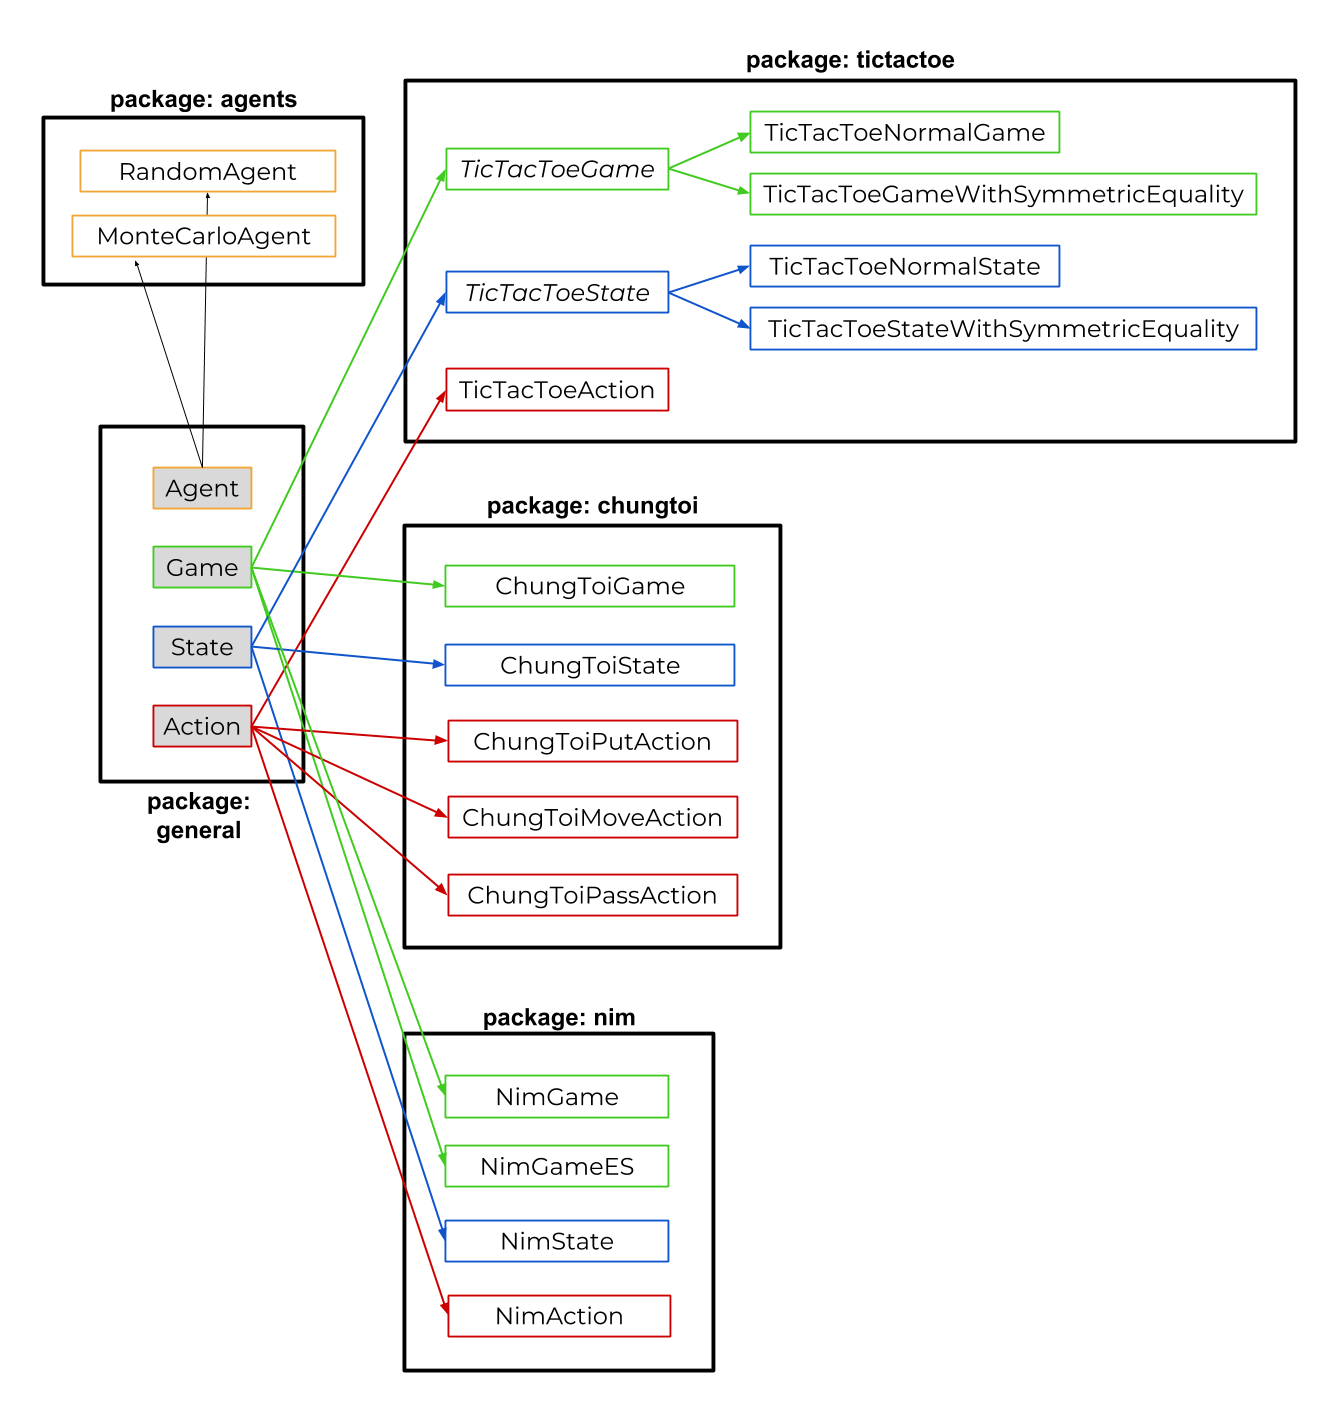
\includegraphics[width=\linewidth]{code_structure.png}
		\caption{Project's code structure. The boxes with a black outline indicate packages, whose names are written in black above them. The filenames with grey backgrounds are interfaces and those with italicised names are abstract classes. An arrow from A to B indicates that B implements or extends A, depending on whether A is an interface or abstract class, respectively. The colourful boxes around each file name indicates which interface it implements (or is) and is intended to visualise inheritance.}
		\label{code-structure}
	\end{center}
\end{figure}

The \emph{general} package contains interfaces for agents, games, states, and actions, and each concrete class in the project implements one of the four interfaces. The interfaces serve as Facades for the implementations, which are often quite complex.

The \emph{tictactoe} package contains an abstract class \emph{TicTacToeGame} that implements the \emph{Game} interface by providing the logic of the game. Two concrete classes, \emph{TicTacToeNormalGame} and \emph{TicTacToeGameWithSymmetricEquality} extend it and all they do is override the constructors in order to initialise the game's state to the right subclass of \emph{TicTacToeState}. Similar to \emph{TicTacToeGame}, \emph{TicTacToeState} is an abstract class that implements the necessary behaviours of a game state, such as providing a list of available actions and producing the result of applying an action to it. It has two concrete subclasses: \emph{TicTacToeNormalState}, which slightly modifies the constructors, and \emph{TicTacToeWithSymmetricEquality}, which implements the symmetry-breaking described in Section \ref{sec:TicTacToeImplementation}.

The \emph{chungtoi} package has three types of actions, so there are three concrete classes that implement the \emph{Action} interface. The logic in \emph{ChungToiState} for producing a list of available actions is more complex than in the other two games due to the number of possible move combinations as well as the two game phases, as described in more detail in Section \ref{sec:ChungToiRules}.

The \emph{nim} package is relatively simple and there are two classes that implement the \emph{Game} interface: \emph{NimGame} and \emph{NimGameES}. The game logic in the latter forces the game to start with a random state-action pair, as required by the Monte Carlo ES algorithm described in Section \ref{sec:MonteCarloAlgorithms}. Further implementation details can be found in Section \ref{sec:NimImplementation}.

The \emph{agents} package has two classes (\emph{RandomAgent} and \emph{MonteCarloAgent}) that implement the \emph{Agent} interface. As Figure \ref{code-structure} clearly shows, the agent implementations are totally independent on the games. That is, agents do not distinguish between different games and only use methods defined in the general interfaces. This means that the \emph{MonteCarloAgent} class, for example, can be used to play all three games. This modularity provides a nice separation of concerns that enables simpler testing and debugging.

The place where everything comes together and all these classes interact is in the \emph{play()} method from the \emph{Game} interface. The method simulates one episode (e.g. one ``game'' of Tic-Tac-Toe) by asking agents to choose actions, giving agents returns returns, and completing other tasks, depending on the specific game.

The independence of the agents and the game implementations makes the project easily extensible to other agents (i.e. learning algorithms) and games. If the reader wanted to test out the MC agent on some other game, Connect Four for example, they would just have to provide appropriate implementations of the \emph{Game}, \emph{State}, and \emph{Action} interfaces. Similarly, if the reader wanted to test out another RL algorithm, Temporal Difference for instance, they would have to  write a single class that implements the \emph{Agent} interface.

In a way, this flexibility is a secondary goal of this project. More concretely, the project provides a framework for testing learning algorithms on games. It can be built on in a variety of ways in order to do further research in the field of RL.


\section{Agents}
\label{sec:Agents}

Two learning agents were implemented: \emph{RandomAgent} and \emph{MonteCarloAgent}.

\emph{MonteCarloAgent} implements the $\epsilon$-soft on-policy MC control algorithm, as discussed in Section \ref{sec:MonteCarloAlgorithms}. In its \emph{chooseAction(State s)} method, it chooses an action according to its policy for states it has encountered in previous games, and randomly otherwise. In its \emph{gameOver()} method it calls two private helper methods \emph{policyEvaluation()} and \emph{policyImprovement()} that update $Q^{\pi}$ and $\pi$, respectively, as described in Section \ref{sec:monteCarloPseudocode}. Hash maps are used to store $Q^{\pi}$ and $\pi$ for constant time access and insertion.

As its name suggests, \emph{RandomAgent} randomly selects an action from the list of available actions at any given state. In total, the logic for this agent is equivalent to one line of code and this agent is only used to play against the MC agent during training.


\section{Tic-Tac-Toe}
\label{sec:TicTacToe}

The first game used in this project is Tic-Tac-Toe. It was chosen because it has a small state space, it is a conceptually simple game that most people are familiar with, and it can be used to investigate the effect of breaking symmetries on a MC agent's performance.


\subsection{Rules}

Although this is a widely-known game, the rules \cite{tic-tac-toe-rules} are still included here for reference and clarity.

First, one of the two players is randomly selected to use X tokens (the other player uses O tokens). These players are referred to as the ``X-player'' and ``O-player'', respectively, and they both have an unlimited number of tokens at their disposal. The game then consists of the two players alternately placing their tokens in empty spaces on a 3x3 grid, starting with the X-player. Figure \ref{tic-tac-toe-grid-example} is an example of a possible state of the grid.

\begin{figure}[htbp]
	\begin{center}
		
\includegraphics[width=50mm]{tictactoe_grid_example.png}
		\caption{Example of a Tic-Tac-Toe grid. Each of the nine cells can be in one of three states: empty, X, or O.}
		\label{tic-tac-toe-grid-example}
	\end{center}
\end{figure}

The game has three possible endings:

\begin{itemize}
	\item \textbf{X-player wins}: three X tokens form a horizontal, vertical, or diagonal row
	\item \textbf{O-player wins}: three O tokens form a horizontal, vertical, or diagonal row
	\item \textbf{Draw}: the grid is filled and neither player has won
\end{itemize}


\subsection{State Space}
\label{sec:TicTacToeStateSpace}

Since each cell has three possible states, there are at most $3^9 = 19683$ states. In practice, strictly fewer than 19,683 possible states can be reached because technically the grid can be filled only with X tokens, with more O tokens than X tokens, or even with a row of three X tokens \emph{and} a row of three O tokens. None of these examples are valid game states so none of them will ever be encountered in a real game.

Preliminary experiments reveal that, in fact, only 4520 states are reachable, without taking into account the four axes of symmetry of a Tic-Tac-Toe grid. If these are taken into account, we find that there are only 640 unique (quotiented by equality by symmetry) reachable states.


\subsection{Implementation}
\label{sec:TicTacToeImplementation}

One of the aims of this project is to investigate the effect of eliminating a game's state symmetries on the Monte Carlo algorithm's learning rate and optimal learning parameters. In the game of Tic-Tac-Toe, a state can be symmetrical with up to seven other states as result of flipping it in the following ways:

\begin{itemize}
	\item horizontal axis
	\item vertical axis
	\item horizontal axis then vertical axis
	\item major diagonal (i.e. top left to bottom right)
	\item major diagonal then horizontal axis
	\item minor diagonal (i.e. top right to bottom left)
	\item minor diagonal then horizontal axis
\end{itemize}

Of course, for some states, the result of some of these flips are the same, which is why a state might have strictly less than seven other symmetrical states.

With this goal in mind, Tic-Tac-Toe was implemented in two ways:

\begin{itemize}

	\item \textbf{``Normal''}:
This version does not break any symmetry and was used as a baseline.

	\item \textbf{``Symmetric Equality''}: 
This version breaks the symmetry between states by considering two objects representing states to be ``equal'' if they are symmetrical.

\end{itemize}

Implementing the desired behaviour for the Symmetric Equality version was not as simple as initially expected. Overriding the \emph{equals()} method inherited from Java's \emph{Object} class was straightforward. However, overriding the inherited \emph{hashCode()} method was tricky.

A Java \emph{HashMap} places key-value pairs in buckets depending on the value returned by calling \emph{hashCode()} on the keys. Thus, if two keys have different hash codes, then they are placed in two different buckets, even if they are ``equal'' according to both of their \emph{equals()} methods. So, two key-value pairs with ``equal'' keys can both end up being stored in a hash map at the same time if they have different hash codes. This is why it was crucial for the \emph{hashCode()} method in \emph{TicTacToeStateWithSymmetricEquality} to produce exactly the same result for symmetrical states. After considering a few solutions, this behaviour was ultimately implemented by silently converting each state to a canonical form in such a way that symmetrical states have the same canonical form. Each state's canonical form is used to compute the state's hash code, which results in all symmetrical states having the same hash code, as required.

In both Tic-Tac-Toe implementations, agents receive a return of 1 for an action resulting a win, -1 for an action resulting in a loss, and 0 for an action resulting in a draw or a non-terminal state.


\section{Chung Toi}
\label{sec:ChungToi}

The second game used in the project is Chung Toi, a more complex version of Tic-Tac-Toe that has been studied in the context of reinforcement learning \cite{chung-toi-rl}. Its state space is larger than that of Tic-Tac-Toe which leads to interesting results.


\subsection{Rules}
\label{sec:ChungToiRules}

The main idea behind Chung Toi \cite{chung-toi-rules} is the same as that behind Tic-Tac-Toe in the sense that the game is played on a 3x3 grid and each player's goal is to get three of their pieces in a row. However, that is the entire extent of their overlap. Although the two games may seem similar, finding a good strategy for Chung Toi is not at all intuitive, unlike in Tic-Tac-Toe.

Before the game begins, one of the two players is randomly selected to use red tokens (the other player uses white tokens). These players are referred to as the ``red player'' and ``white player'', respectively. Each player has three tokens at their disposal and each token can be used in two possible orientations, as shown in Figure \ref{chung-toi-tokens}.

\begin{figure}[htbp]
	\begin{center}
		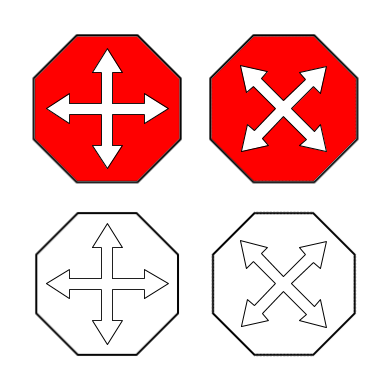
\includegraphics[width=40mm]{chung_toi_tokens.png}
		\caption[Chung Toi tokens]{Red and white Chung Toi tokens in both possible orientations. The tokens in these orientations are referred to as: red-straight (top-left), red-diagonal (top-right), white-straight (bottom-left), and white-diagonal (bottom-right).}
		\label{chung-toi-tokens}
	\end{center}
\end{figure}

The game consists of the players alternately making a move, starting with the red player. Throughout the game, the red player can only move red tokens and the white player can only move white tokens. The game has two phases and both players start in Phase 1. Once a player places all three of their tokens, that player proceeds to Phase 2. The following actions are available in each phase:

\begin{itemize}

	\item \textbf{Phase 1}
		\begin{itemize}
			\item Place a token (in either orientation) in an empty grid cell
			\item Pass
		\end{itemize}

	\item \textbf{Phase 2}
		\begin{itemize}
			\item Slide a token on the grid in the direction of any of the arrows on that token. When the token reaches the final cell, it can be rotated to switch its orientation if the player chooses to do so. \emph{(Note: all grid cells in the path from the original cell to the final cell must be empty, meaning that the token cannot ``jump'' over other tokens)}
			\item Rotate one token to switch its orientation
			\item Pass
		\end{itemize}

\end{itemize}

If both players pass on consecutive turns at any point, the game ends and is declared a draw. Otherwise, the game continues until one of the players makes their tokens form a horizontal, vertical, or diagonal row and that player is declared the winner. The orientation of the three tokens in the row does not matter.

Figure \ref{chung-toi-grid-example} is an example of a possible state of the grid.

\begin{figure}[htbp]
	\begin{center}
		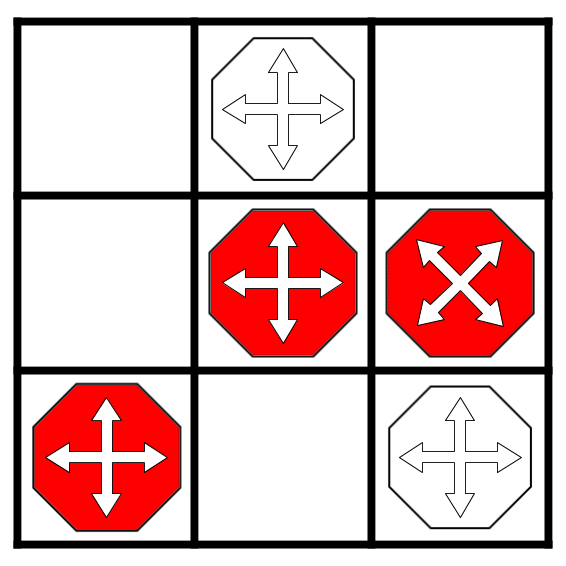
\includegraphics[width=50mm]{chung_toi_grid_example.png}
		\caption{Example of a Chung Toi grid. Each of the nine cells can be in one of five states: empty, red-straight, red-diagonal, white-straight, or white-diagonal.}
		\label{chung-toi-grid-example}
	\end{center}
\end{figure}


\subsection{State Space}

Since each cell has five possible states, there are at most $5^9 = 1,953,125$ states. For the same reasons outlined in Section \ref{sec:TicTacToeStateSpace}, strictly fewer than this many states are reachable in practice and even fewer are unique with respect to the four axes of symmetry.


\subsection{Implementation}

A standard implementation of Chung Toi was developed for this project. It enables two agents to play the game, exactly as described above.

The role of Chung Toi in this project was to learn more about the effect of the MC learning parameter $\varepsilon$ on an agent's learning rate and winning rate. Chung Toi has roughly 100 times more states than Tic-Tac-Toe, which is expected to have an effect on the optimal value of $\varepsilon$ and therefore the MC agent's learning rate. It has the same axes of symmetry as Tic-Tac-Toe, so similar results would be expected from a Chung Toi implementation that breaks symmetries. For this reason, such an implementation was not developed to reduce redundancy and instead only a normal implementation with all symmetrical states present was developed.

Just like in Tic-Tac-Toe, agents receive a return of 1 when they win, -1 when they lose, and 0 when the game ends in a draw or the game has not yet ended.


\section{Nim}
\label{sec:Nim}

The third game used in the project is Nim, a simple game with an interesting mathematical theory behind it \cite{nim-rules}. It has a large number of variations and can be configured in many ways, so its state space can vary widely. For the purposes of this project, a ``small'' version of the game is used in order to reduce the running time of the experiments.


\subsection{Rules}

The general idea of Nim \cite{nim-rules} is that two players alternately remove objects from several piles. The first player is chosen randomly and then on each turn, a player can remove any number of objects from any one of the piles. Each player must remove at least one object on each turn. The game ends when all the piles are empty.

Which player wins depends on which version of the game is being played. In the ``normal play'' version the last move is the winning move, whereas in the ``mis\`ere'' version the player who moves last loses \cite{winning-ways-math-plays}. The mis\`ere version is implemented in this project.


\subsection{State Space}

As explained in Section \ref{sec:NimImplementation}, the ``small'' version of Nim used in this project  consists of three piles, initially with seven objects each. Since each pile can have between zero and seven objects, inclusive, there are $8^3 = 512$ possible states.


\subsection{Implementation}
\label{sec:NimImplementation}

Nim is traditionally played with three piles of objects. The first of two versions of Nim implemented in this project is standard and initialises all piles with a fixed number of objects. In particular, in order to keep the state space relatively small, all three piles start off with seven objects.

A second version of Nim was implemented since the game is well-suited to investigating the performance of Monte Carlo ES. This is because instead of initialising all piles with a fixed number of objects, all piles can be initialised with random numbers of objects.

In this second implementation, piles are initialised with a random number of objects between zero and seven, in such a way that at least two piles are non-empty. This last condition was necessary because if all piles are empty or if there is only one non-empty pile and the other agent goes first and removes all the objects, then the game ends and the MC agent must receive a return without having chosen any action. This creates problems in the policy improvement phase of the algorithm since there is an outstanding return relative to the number of actions taken (i.e. zero).

Since the concept of exploring starts relies on games starting with random state-action pairs, the implementation of the MC agent (as well as the \emph{Agent} interface and random agent) had to be modified and a slightly modified version of Nim was created. This is because in addition to randomly initialising the piles, an action has to be randomly selected. Then, the agent that is randomly selected to go first has to be forced to choose that random action. In this way, in the limit of infinitely many games, all actions from all states are explored and the agent is able to determine the overall best return it can receive from each state.

At the end of the game, the winner receives a return of 1 and the loser receives a return of -1. Throughout the rest of the game, both players receive returns of 0 for all their actions.


%------------------
\chapter{Results \& Analysis}

This section describes the outcomes of a variety of experiments and discusses why these outcomes were expected, or unexpected, and what can be learned from them.


\section{Types of Experiments}
\label{sec:experiment-types}

Two types of experiments were used to investigate the behaviour of the MC agent when playing games:

\begin{itemize}

	\item \textbf{``Epsilon'' Experiment}: This type of experiment iterates through all values of epsilon in a particular range (see Section \ref{sec:epsilon-precision}) and makes a MC agent (initialised with each value of epsilon) play a specific game against another agent a fixed number of times for training and then another fixed number of times for testing. Then it records the results (i.e. wins, losses, draws) for each value of epsilon during the testing phase in a CSV file. Thus, it is possible to produce graphs with the tested values of epsilon on the x-axis and the number of testing episodes resulting in a win, loss, and draw on the y-axis. These graphs are used to determine the optimal value of epsilon for a particular game and to decide which valuesof epsilon to use for ``convergence'' experiments.

	\item \textbf{``Convergence'' Experiment}: This type of experiment makes a MC agent (initialised with a particular value of epsilon) play a specific game against another agent a fixed number of times. Throughout the process, it records the cumulative results (i.e. wins, losses, draws) at regular intervals, as more and more episodes are played, in a CSV file. Thus, it is possible to plot the winning rate against the cumulative number of training episodes. These graphs are used to visualise the convergence rate of a MC agent's policy when using a specific value of epsilon. A deeper analysis of the significance of measuring convergence and the meaning of the winning rates when the policy converges can be found in Section \ref{sec:policy-optimality}.

\end{itemize}

The data from running these experiments on different games and with a MC agent playing testing and training episodes against other agents different numbers of times was combined to produce a number of interesting graphs that reveal interesting properties of the MC control algorithm.


\section{Number of Training Episodes}

An important decision made as part of the design and execution of these experiments was the number of training and testing episodes to use for each game. Two different approaches were used: one for Tic-Tac-Toe and Nim since they have relatively small state spaces ($<$5,000 states) and one for Chung Toi since it has a very large state space.

For Tic-Tac-Toe and Nim, a structured process of trial-and-error was used to determine roughly how many episodes a MC agent needed to play in order for it to encounter all possible states for at least \emph{some} values of epsilon. This was done by training an agent with 100, 1,000, 10,000, and 100,000 games for each value of epsilon and inspecting the size of its policy in each case. A particular number of training episodes was deemed suitable if it resulted in a non-trivial proportion of the values of epsilon causing the agent to reach all possible states (4520 states in the case of Tic-Tac-Toe and 511 states in the case of Nim). These values of epsilon were always large (i.e. close to 1.0) because as epsilon gets larger, the agent is expected to encounter more and more states because it chooses actions at random increasingly often.

The results indicated that 1,000 episodes sufficed for Nim and 10,000 episodes sufficed for Tic-Tac-Toe. These numbers differ by one order of magnitude, which matches the difference in the number of states the two games have. So, the number of training episodes used for Nim started at 1,000 and was repeatedly doubled until 128,000 (inclusive) and similarly for Tic-Tac-Toe it started at 10,000 and was repeatedly doubled until 1,280,000 (inclusive). For the sake of simplicity, the number of testing episodes was 1,000 for Nim and 10,000 for Tic-Tac-Toe.

This process was reasonable for Tic-Tac-Toe and Nim because they have relatively small state spaces and so it was possible to make an agent play enough episodes for it to encounter all possible states in a sensible amount of time. Chung Toi, on the other hand, has roughly 100 times as many states as Tic-Tac-Toe and it was not feasible to make an agent play millions or billions of games to reach them all.

It is worth making a short digression to point out that this is one of the limitations of Monte Carlo algorithms and is one of the main reasons they are not used heavily in practice where reinforcement learning tasks have very large state spaces. In particular, since the agent learns only from its experience, without attempting to draw any conclusions about states it has not encountered, its success and therefore usefulness for tasks with a lot of states becomes rather limited. This is why ``pure'' Monte Carlo algorithms (i.e. algorithms that do not combine Monte Carlo techniques with other techniques like dynamic programming) tend to be applied only to simple tasks with small state spaces and are generally used for educational rather than practical purposes. On the other hand, algorithms like Temporal Difference learning, as briefly discussed in Section \ref{sec:learning-algorithms}, are much better suited to situations like these where the state space cannot be fully explored. Nevertheless, it was interesting to put a MC agent to the test with Chung Toi to see what success rate it could achieve.

Since there was no clear way of determining a reasonable number of training and testing episodes for Chung Toi, the numbers used for Tic-Tac-Toe were also used for Chung Toi. This meant that experiments could be run in a reasonable amount of time (i.e. on the order of hours rather than days or weeks).


\section{Epsilon Precision}
\label{sec:epsilon-precision}

Another decision was which values of epsilon to use for the epsilon experiments. The graphs with the experiment results have the values of epsilon on the x-axis and the win/loss/draw rates on the y-axis as a percentage of the testing episodes. Thus, in order to have a relatively smooth graph, epsilon values were chosen at regular intervals. Since epsilon can range from 0.0 to 1.0, the size of these intervals (aka. the epsilon precision, as defined in Section \ref{sec:Terminology}) was chosen to be 0.01. Using 0.1 made it difficult to compare the results of epsilon experiments where the curves were similar. Using 0.05 was a bit better, but 0.01 was good because it provided a clear visualisation of the differences between experiments without saving unnecessary amounts of data.

As with any decision like this one, there is a point ``of diminishing returns'' after which having more detailed data does not enable more meaningful conclusions to be drawn. Thus, for the purposes of this project, the line was drawn at an epsilon precision of 0.01.


\section{Optimal Value of $\varepsilon$}
\label{sec:optimal_epsilon}

It is not unreasonable to expect each game to have a specific value of epsilon that results in the fastest convergence of the MC agent's policy. If this was the case, then one would expect the graph of the winning rate produced by an epsilon experiment with $\varepsilon$ ranging from 0.0 to 1.0 (inclusive) to be convex with a global maximum. This belief is vaildated by running an epsilon experiment on any game for some number of training episodes. For example, Figure \ref{chung-toi-epsilon-160ktrain-10ktest} displays the results of 10,000 Chung Toi testing episodes after 160,000 training episodes.

\begin{figure}[htbp]
	\begin{center}
		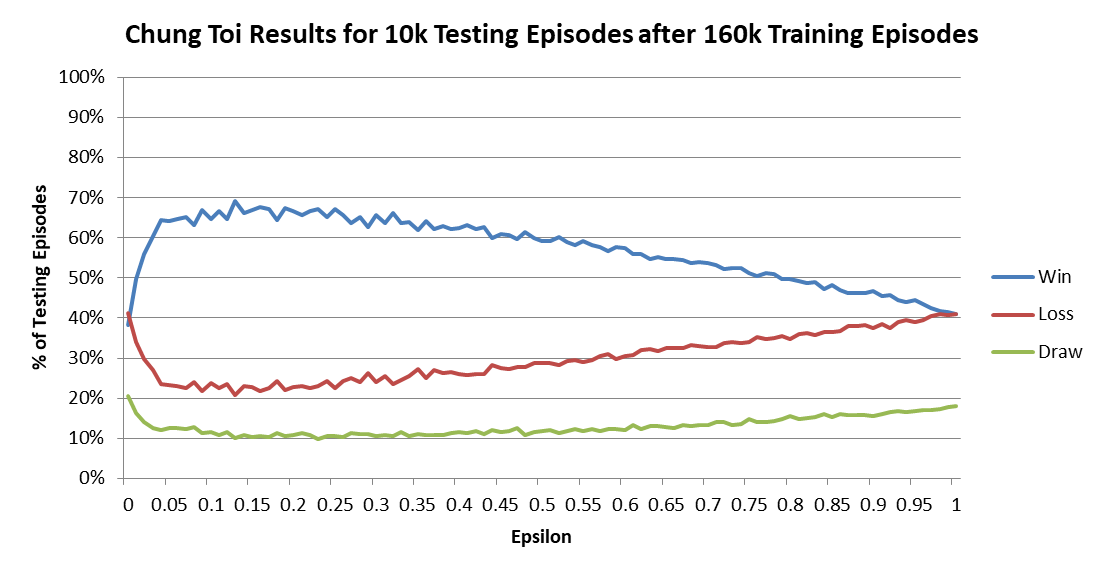
\includegraphics[width=\linewidth]{ChungToi_EpsilonResults_160kTrainingGames_10kTestingGames.png}
		\caption{MC agent's performance on 10,000 Chung Toi testing episodes after 160,000 training episodes. There is a global maximum at $\varepsilon \approx 0.15$, which suggests that this is the best value of epsilon to use, at least for these numbers of training and testing episodes.}
		\label{chung-toi-epsilon-160ktrain-10ktest}
	\end{center}
\end{figure}

However, with some experimentation it becomes clear that there is another key factor in the equation: the number of training episodes. If a game is judged based on the results of a single epsilon experiment (which uses some number of training episodes), the belief that each game has an optimal epsilon value seems to be true. However, when many epsilon experiments that use different numbers of training episodes are considered, an interesting relationship between the number of training episodes and the optimal value of epsilon is uncovered. Figure \ref{epsilon-win-comparisons} demonstrates this relationship for all three games.

\begin{figure}[htbp]
    \centering
    \subfigure[Normal Tic-Tac-Toe]{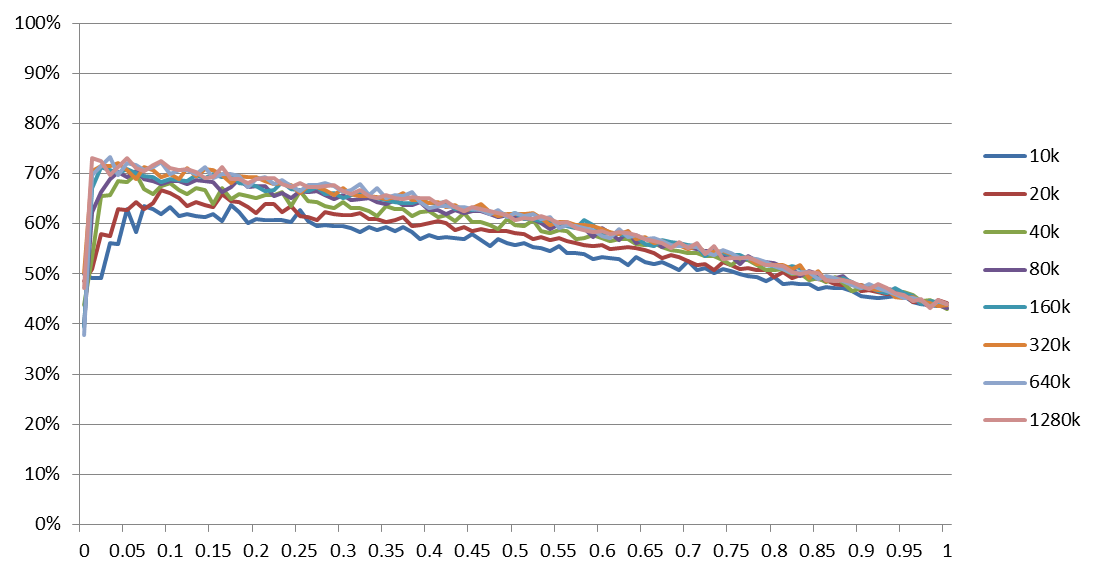
\includegraphics[width=0.75\linewidth]{TicTacToeNormal_EpsilonResults_Wins_Comparison_no_title.png}}
    \subfigure[Chung Toi]{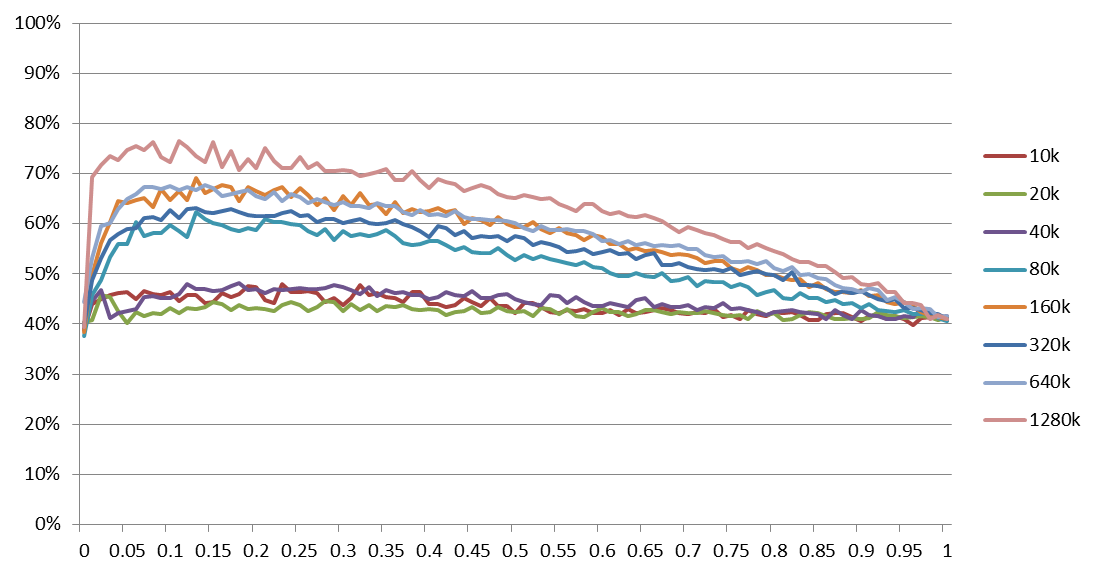
\includegraphics[width=0.75\linewidth]{ChungToi_EpsilonResults_Wins_Comparison_no_title.png}}
    \subfigure[Nim]{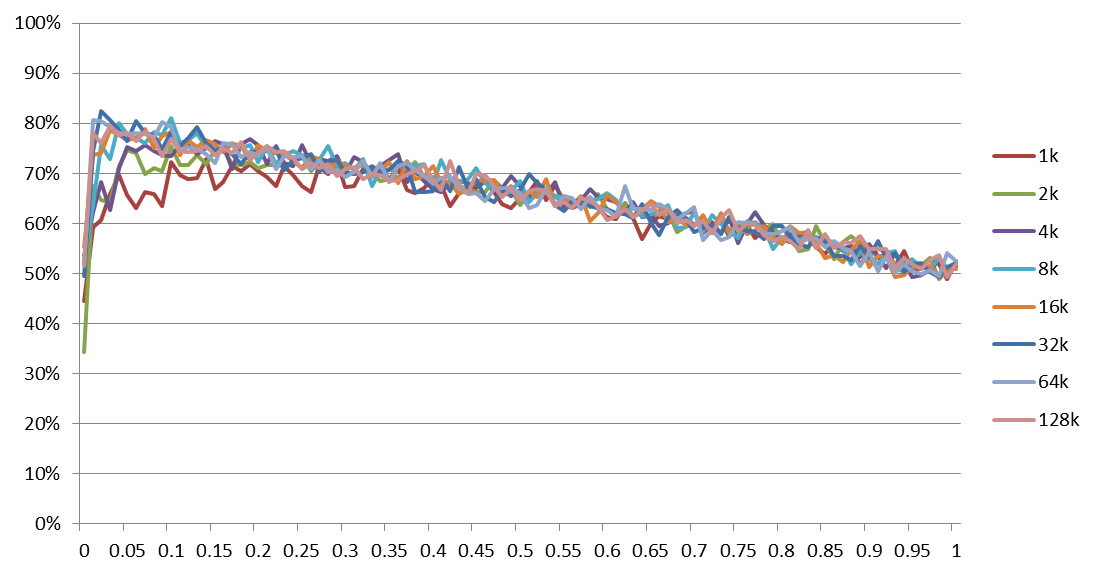
\includegraphics[width=0.75\linewidth]{Nim_EpsilonResults_Wins_Comparison_no_title.png} \label{fig:nim_win_comparison}}
    \caption{Comparison of a MC agent's winning rate for 10,000 testing episodes after different numbers of training episodes, for each of the three games. In each graph, the x-axis shows the value of epsilon, the y-axis shows the percentage of testing episodes won, and the legend entries indicate the number of training episodes the agent played before testing.}
    \label{epsilon-win-comparisons}
\end{figure}

Thus, as the number of training episodes increases, the highest winning rate increases and the value of epsilon that produces the highest winning rate (``optimal'' value of epsilon) decreases. In particular, if we look at the optimal value of epsilon for each number of training episodes tried and plot these results for any game, we get a graph that looks like Figure \ref{nim-training-vs-opt-epsilon}. This shows that there is an inverse relationship between the two. This means that if there are no time or computational limitations and therefore a lot of training episodes can be played, a smaller value of epsilon will produce a higher win rate. In fact, as the number of training episodes approaches infinity, the optimal value of epsilon approaches zero. However, if the MC agent can only play a limited number of training episodes due to time or computational limitations, then a larger value of epsilon will produce better results.

\begin{figure}[htbp]
	\begin{center}
		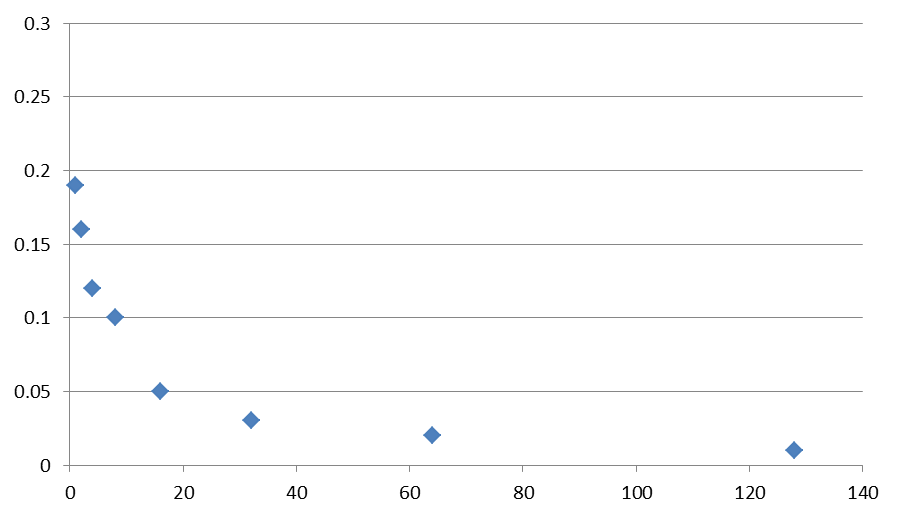
\includegraphics[width=\linewidth]{Nim_OptimalEpsilon_vs_Training.png}
		\caption{Graph of the optimal epsilon value for different numbers of Nim training episodes, showing an inverse relationship. These values were extracted from the CSV files produced by the epsilon experiments, where each experiment used a different number of training episodes -- call this $N$. The optimal value of epsilon for each experiment is the value for which the MC agent trained for $N$ episodes using that value of epsilon had the highest winning rate during the testing session. More intuitively, the datapoints correspond to the global maxima of each of the curves in \ref{fig:nim_win_comparison}. }
		\label{nim-training-vs-opt-epsilon}
	\end{center}
\end{figure}

This behaviour makes sense and should, in fact, be expected because of the role of $\varepsilon$ in the Monte Carlo control algorithm. As discussed in Section \ref{sec:MonteCarloAlgorithms}, $\varepsilon$ is used during policy improvement. In particular, the probability of choosing an action (other than the best action encountered so far) is $\frac{\varepsilon}{N}$ where $N$ is the number of available actions. On the other hand, the probability of choosing the best action encountered so far is  $1 - \epsilon + \frac{\varepsilon}{N}$. Thus, as $\varepsilon$ approaches 0, the probability of choosing the best action encountered so far approaches one.

A larger value of $\varepsilon$ benefits an agent in the short-term because it speeds up learning. This is because a larger $\varepsilon$ value corresponds to more exploration, relative to exploitation, which means the best actions will be found faster. Thus, when few training episodes can be played, a value of $\varepsilon$ closer to 1 is better. However, it is disadvantageous in the long-term because even though the agent knows which actions produce the largest returns, the agent will still be forced to choose other sub-optimal actions relatively often. So, when a large number of training episodes can be played, a value of $\varepsilon$ closer to 0 is better.

Overall, there is no single value of $\varepsilon$ that maximises an agent's performance in a particular game. However, for any \emph{specific} number of training episodes, there \emph{is} a value that results in the best winning rate by striking the right balance between exploration and exploitation for \emph{that} amount of training.

Of course, the same number of training episodes will have different optimal $\varepsilon$ for games with different state space sizes and even game lengths (i.e. average number of actions until the game ends). The key point, however, is still the same and it is that a training episode number and epsilon combination that works well for one game is unlikely to work as well for another and so each game needs to be studied separately.


\section{Convergence to the Optimal Policy}
\label{sec:convergence-results}

In the context of training a MC agent to play a game, the ``speed'' at which the agent's policy converges is the number of training episodes the agent needs until its policy $\pi$ converges. Naturally, this varies depending on the value of $\varepsilon$ used by the agent.

As described in Section \ref{sec:experiment-types}, convergence experiments provide the data needed to compare different values of $\varepsilon$ and to analyse the speed of convergence. Convergence experiments produce the proportions of a MC agent's wins and losses (and draws, if applicable) at regular intervals during a training session, using a specific value of epsilon. Thus, by plotting the proportions of wins, we see how quickly the policy changes. Convergence experiments do not involve any testing episodes because their goal is to analyse the algorithm during training in order to gain insight into what an appropriate number of training episodes is for a particular game.

The policy of the MC agent only converges to the theoretically optimal policy in the limit of infinitely many training episodes \cite{rl-book}. Since running infinitely many episodes is naturally infeasibly, 100,000 training episodes are run in the convergence experiments and the resulting graphs are inspected to see how long it takes for the winning rate to stabilise.

It might also be natural to define some notion of convergence. For instance, one might consider the policy to have converged after $x$ training episodes if the agent's winning rate changes by less than 0.1\% after $x$ training episodes compared to after $x+1000$ training episodes. This technique was trialled, but the results did not provide any additional insight relative to visual inspection and comparison of the convergence experiment graphs, so they are omitted.

As we saw earlier in Figure \ref{fig:nim_win_comparison}, the agent's winning rate when playing Nim changes quite a bit as the number of training episodes increases. The best way to gain an intuition of how the policy converges for different epsilon value is to run convergence experiments with a few different values. Figure \ref{nim-convergence-comparison} shows the results of experiments run for $\varepsilon = 0.01, 0.02,..., 0.64$.

\begin{figure}[htbp]
	\begin{center}
		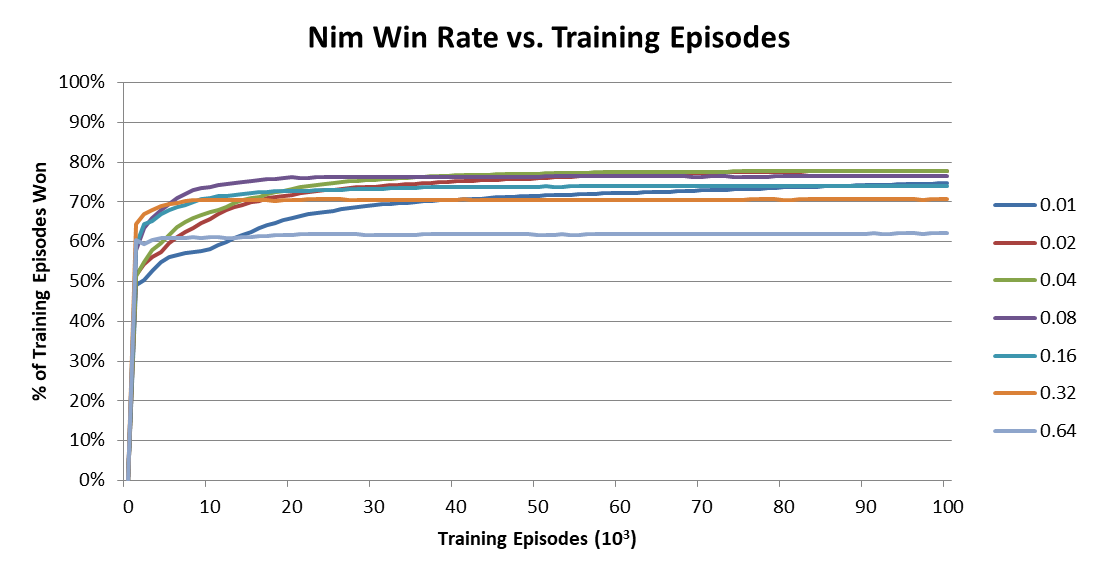
\includegraphics[width=\linewidth]{Nim_PerformanceResults_Comparison_001_to_064.png}
		\caption{Changes in the agent's winning rate for Nim as the number of training episodes increases, for different values of epsilon. The legend entries indicate the values of epsilon used. The highlighted datapoints indicate the places where the policy converges.}
		\label{nim-convergence-comparison}
	\end{center}
\end{figure}

Figure \ref{nim-convergence-comparison} does an excellent job of illustrating the impact of the value of epsilon on the winning rate. There is a very clear trend: as epsilon increases, the policy converges faster (i.e. after fewer training episodes). Also, for the most part, as epsilon increases, the stabilised winning rate decreases -- this trend is particularly clear for the larger value of epsilon.

In fact, Figure \ref{nim-convergence-comparison} also turns out to be another way of visualising the balance between the magnitude of epsilon and the number of training episodes that maximises the agent's winning rate. Suppose that performance experiments are run for all values of epsilon from 0 to 1, inclusive at intervals of 0.01 and that all the curves are plotted on the same graph. Consider a vertical ``slice'' of the graph -- namely the winning rate for each value of epsilon after a specific number of training episodes, say 8,000. This slice is actually a projection of the graph of the winning rates from an epsilon experiment for 8,000 training episodes onto the y-axis. Figure \ref{nim-epsilon-flattening} gives a visualisation of such a projection.

\begin{figure}[htbp]
    \centering
    \subfigure[Nim winning rate for 1,000 testing episodes after 8,000 training episodes]{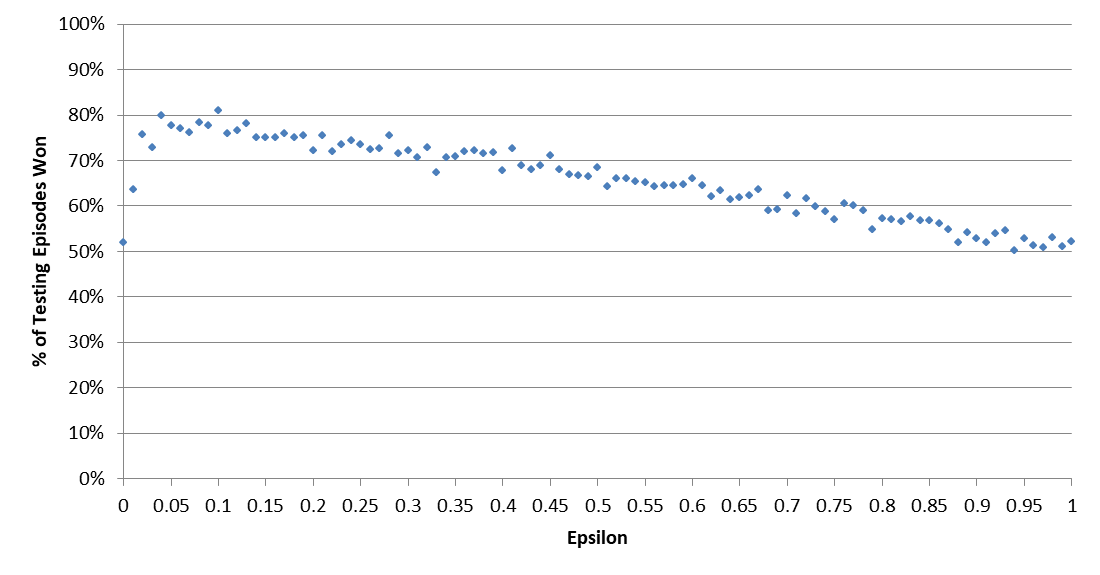
\includegraphics[height=0.15\paperheight]{Nim_EpsilonResults_8kTrainingGames_1kTestingGames.png} \label{nim-8k-epsilon-results}}
    \subfigure[Results projected onto y-axis]{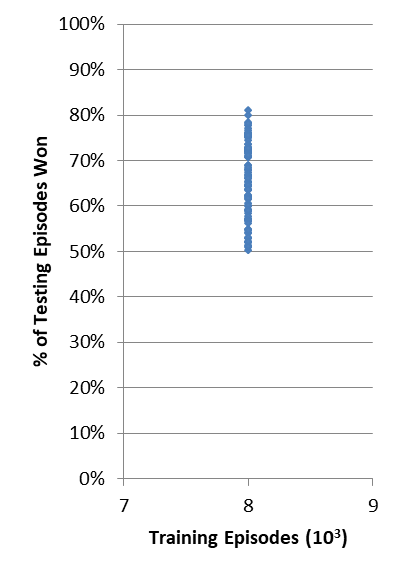
\includegraphics[height=0.15\paperheight]{Nim_EpsilonResults_8kTrainingGames_1kTestingGames_Flattened.png}  \label{nim-8k-epsilon-results-flattened}}
    \caption{Flattening of Nim epsilon experiment results. \ref{nim-8k-epsilon-results} shows the winning rate from a Nim epsilon experiment for 8,000 training episodes. \ref{nim-8k-epsilon-results-flattened} shows the same results, but projected onto the y-axis. Each data point corresponds to a different value of epsilon.}
    \label{nim-epsilon-flattening}
\end{figure}

Each slice corresponds to the results of some epsilon experiment, so the same simple equation is used  in both cases to choose which epsilon to use for a fixed number of training episodes. Specifically:

\begin{equation}
	\varepsilon^{optimal} = \argmax_{\varepsilon} WinningRate(\varepsilon)
\end{equation}

Overall, these results verify what was uncovered in Section \ref{sec:optimal_epsilon}. Specifically, the choice of epsilon depends on how many training episodes can be played. For few episodes, larger values of epsilon are better since they converge to their maximal winning rate quickly. For a large number of episodes, smaller value of epsilon are preferable because they provide a better maximal winning rate once they converge.


\section{Monte Carlo with Exploring Starts}

The game that is most conducive to applying the Monte Carlo with Exploring Starts (Monte Carlo ES) algorithm is Nim because it is easy to create a random starting state. Since Monte Carlo ES does not have any learning parameters like $\varepsilon$, the only relevant type of experiment is a convergence experiment. Normally, a convergence experiment takes a value of $\varepsilon$ as an argument, but since such a value is not used by an agent that implements the exploring starts algorithm, the argument is ignored. Thus, the only experiment parameter that can be modified is the total number of training episodes. For consistency with the other Nim experiments, the convergence experiment for Nim with ES was run 100,000 times and the results can be seen in Figure \ref{nim-convergence-comparison-with-ES}.

\begin{figure}[htbp]
	\begin{center}
		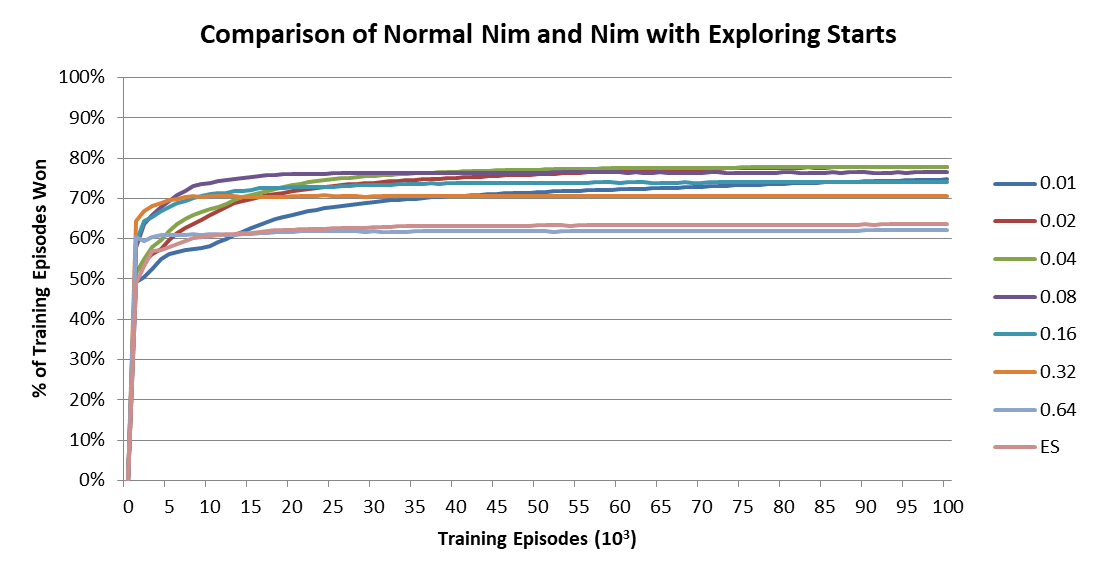
\includegraphics[width=\linewidth]{Nim_PerformanceResults_Comparison_001_to_064_and_ES.png}
		\caption{Comparison of the results of convergence experiments for Nim with ES and normal Nim with different values of epsilon. This is identical to the graph in Figure \ref{nim-convergence-comparison} except that the curve for the Monte Carlo ES algorithm is superimposed.}
		\label{nim-convergence-comparison-with-ES}
	\end{center}
\end{figure}

As we can see, Monte Carlo ES performs similarly to Monte Carlo with a relatively large value of epsilon (like $\varepsilon$ = 0.64 in Figure \ref{nim-convergence-comparison-with-ES}). This seems reasonable because as epsilon approaches 1, the agent chooses actions randomly more and more often. Thus, the agent is increasingly likely to choose actions that lead to suboptimal or losing states (i.e. states where the other player can win in their next move), regardless of whether or not they know better. In a similar way, Monte Carlo ES forces the agent into certain states (right at the start of each episode), many of which are sub-optimal or losing states. This element of randomness when Monte Carlo ES determines the starting state appears to have a similar effect to the element of randomness that the on-policy $\varepsilon$-soft MC algorithm exhibits when epsilon is large.

Clearly, Monte Carlo ES does converge to some policy, but it is clear that there are better policies since many values of epsilon cause an on-policy $\varepsilon$-soft MC agent to converge to a policy with a higher winning rate.


\section{Effect of Eliminating Symmetry}

Tic-Tac-Toe is used to study the effect of eliminating all axes of symmetry from a game on a MC agent's performance. As discussed in Section \ref{sec:TicTacToeImplementation}, each Tic-Tac-Toe state can be symmetrical with up to seven other states. The game has four axes of symmetry (horizontal, vertical, and two diagonals) and reflecting states in one or more of them produces all possible reflections and rotations. The ``normal'' Tic-Tac-Toe implementation does not implement any symmetry-breaking, whereas the ``symmetric equality'' (SE) Tic-Tac-Toe implementation breaks all symmetry between states -- these are discussed in more detail in Section \ref{sec:TicTacToeImplementation}.

Naturally, an implementation that breaks symmetries should be expected to perform better because it can combine its knowledge about symmetrical states and therefore produce a more accurate estimate $Q^{\pi}$ of the action-value function. This intuition is confirmed by running epsilon experiments for different numbers of training episoides for both normal Tic-Tac-Toe and SE Tic-Tac-Toe and the results are shown in Figure \ref{fig:tictactoe-normal-vs-symmetric-equality-epsilon}.

\begin{figure}
    \centering

    \subfigure[10,000 training episodes]{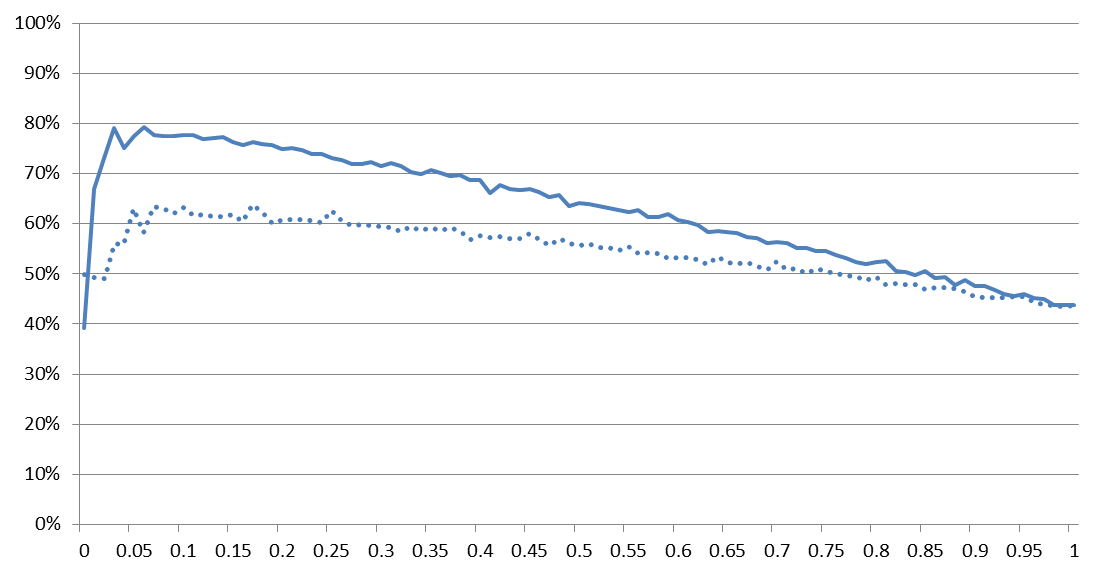
\includegraphics[width=0.49\linewidth]{TicTacToe_Normal_Vs_Symmetric_Equality_10k.png} \label{ttt-n-vs-se-10k}}
    \subfigure[20,000 training episodes]{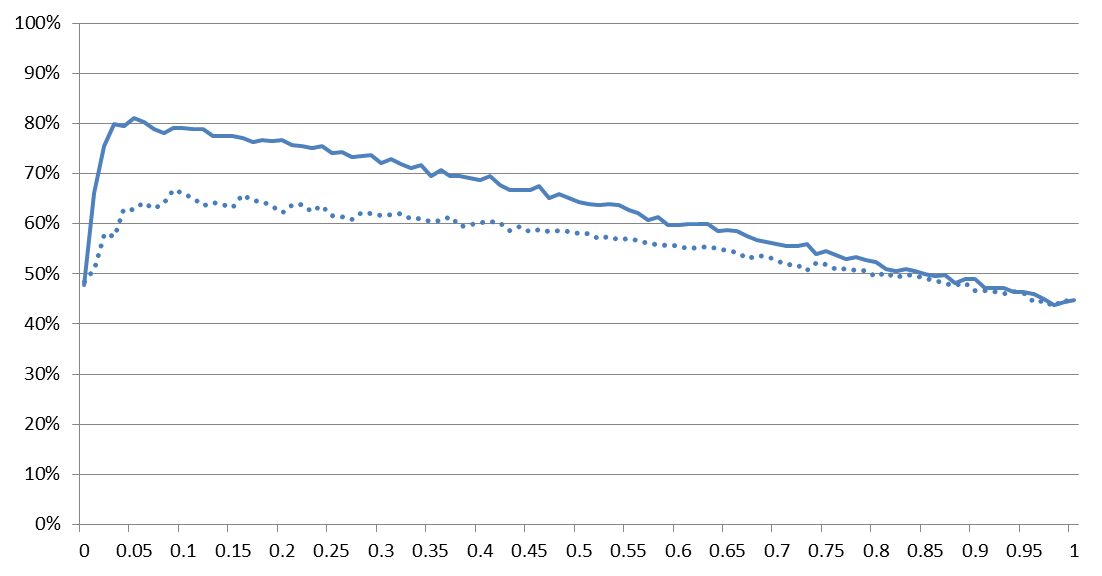
\includegraphics[width=0.49\linewidth]{TicTacToe_Normal_Vs_Symmetric_Equality_20k.png}}
    \subfigure[40,000 training episodes]{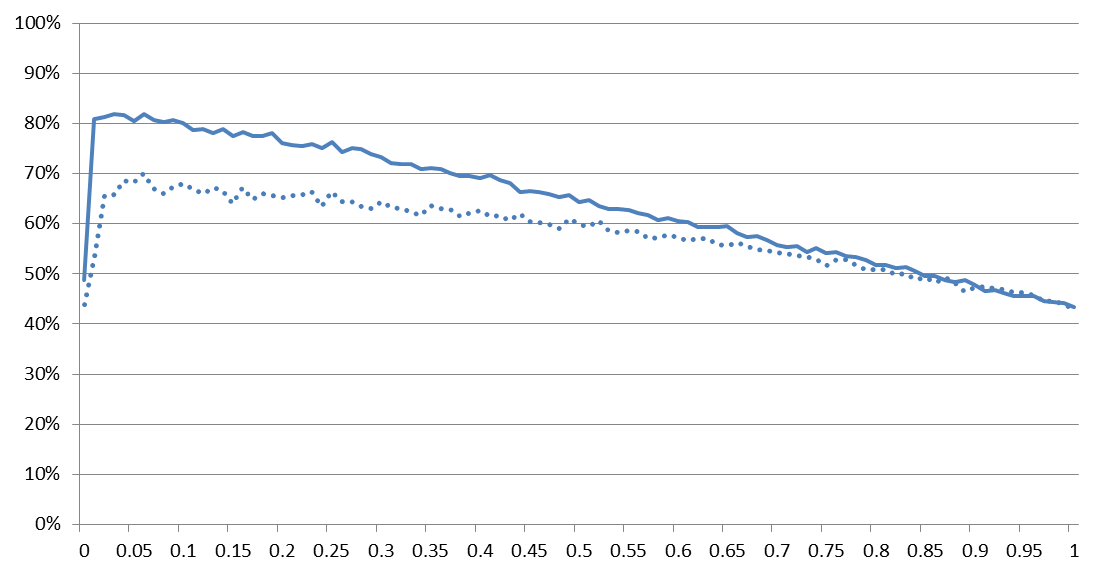
\includegraphics[width=0.49\linewidth]{TicTacToe_Normal_Vs_Symmetric_Equality_40k.png}}
    \subfigure[80,000 training episodes]{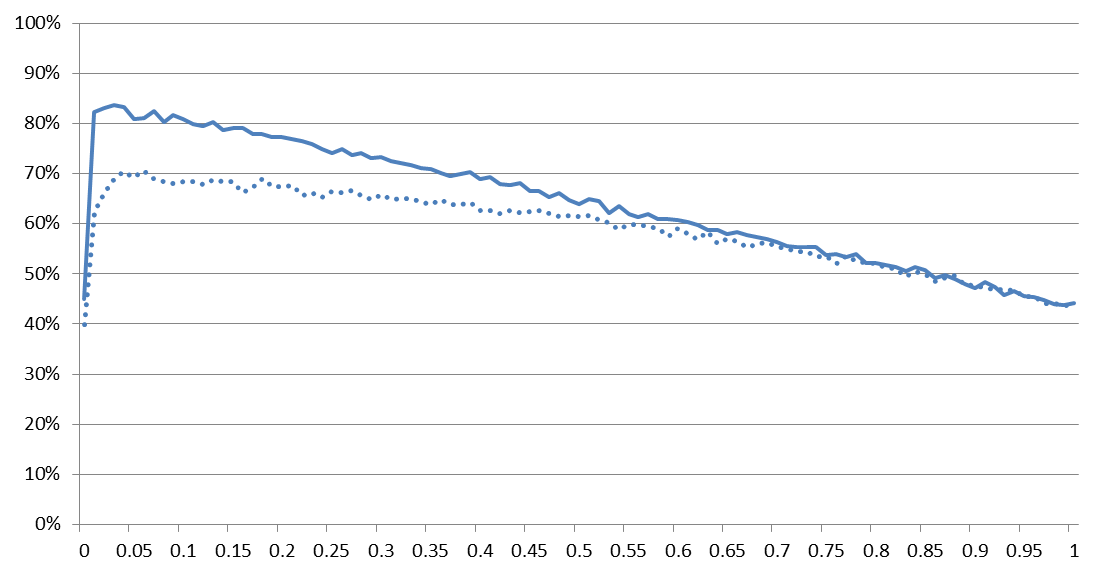
\includegraphics[width=0.49\linewidth]{TicTacToe_Normal_Vs_Symmetric_Equality_80k.png}}
    \subfigure[160,000 training episodes]{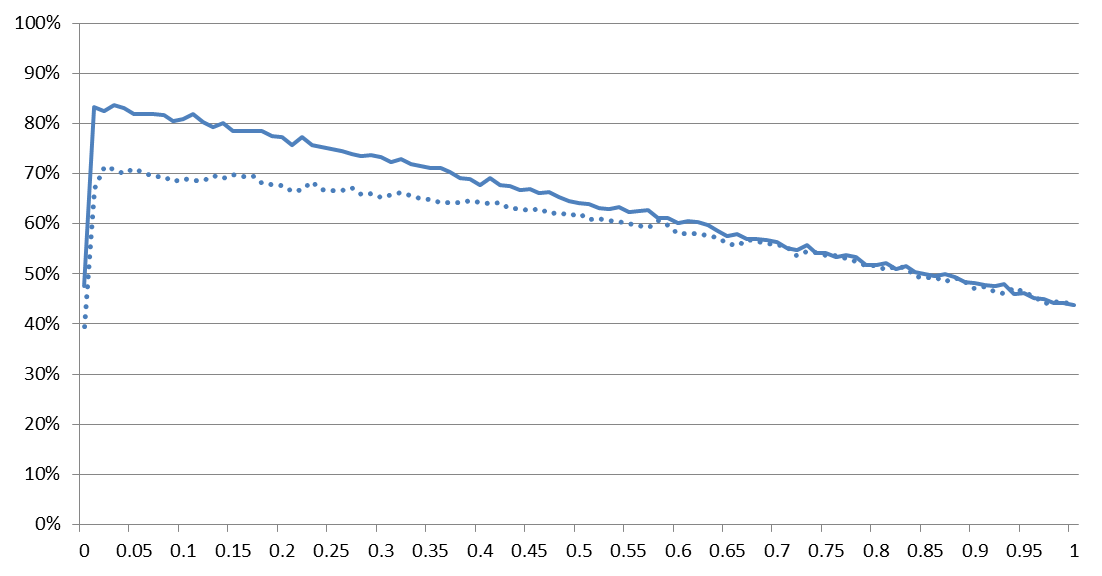
\includegraphics[width=0.49\linewidth]{TicTacToe_Normal_Vs_Symmetric_Equality_160k.png}}
    \subfigure[320,000 training episodes]{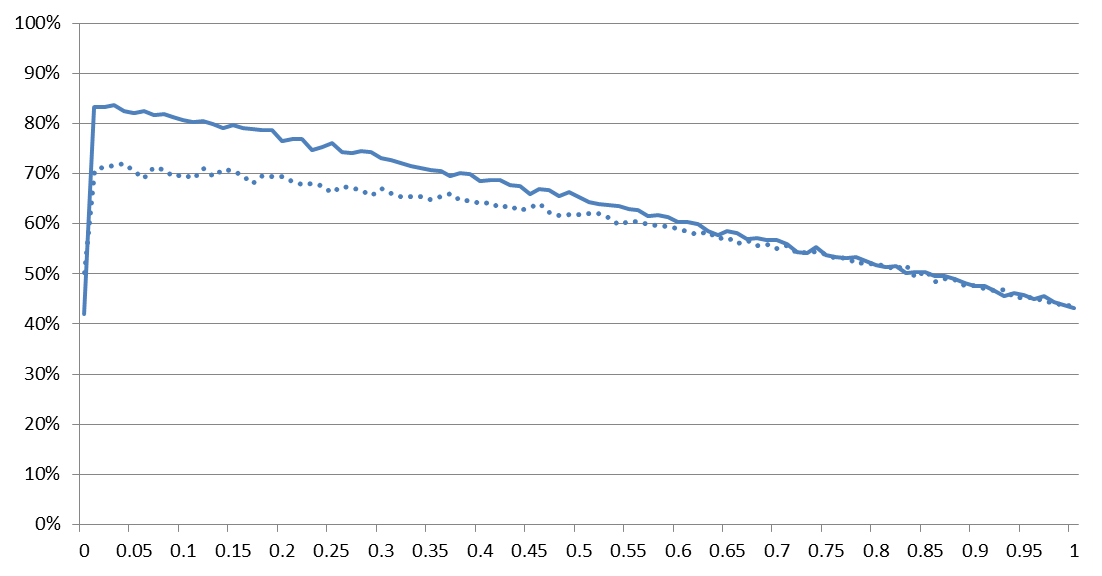
\includegraphics[width=0.49\linewidth]{TicTacToe_Normal_Vs_Symmetric_Equality_320k.png}}
    \subfigure[640,000 training episodes]{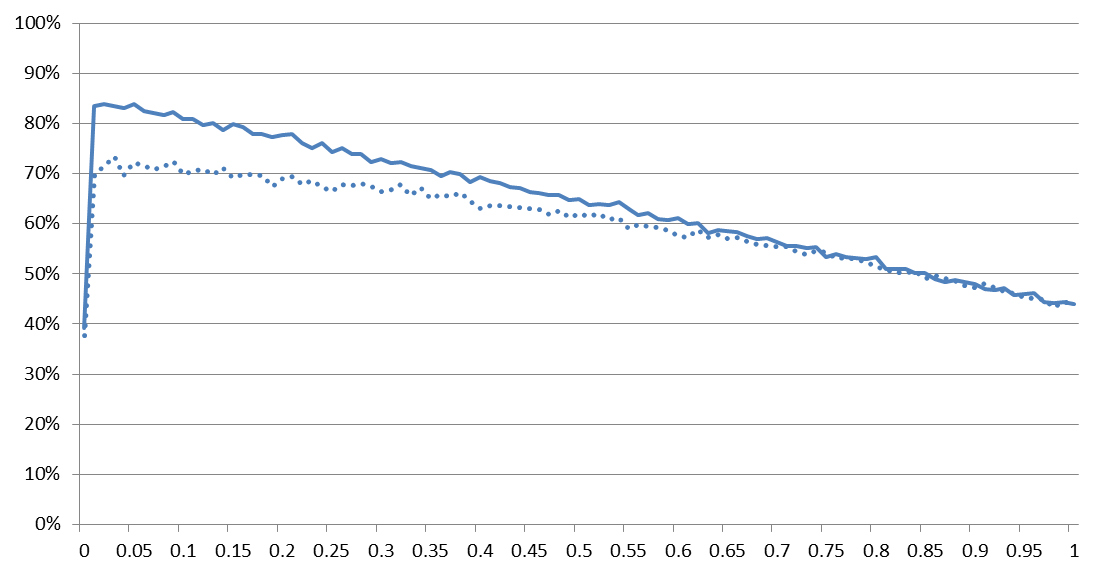
\includegraphics[width=0.49\linewidth]{TicTacToe_Normal_Vs_Symmetric_Equality_640k.png}}
    \subfigure[1,280,000 training episodes]{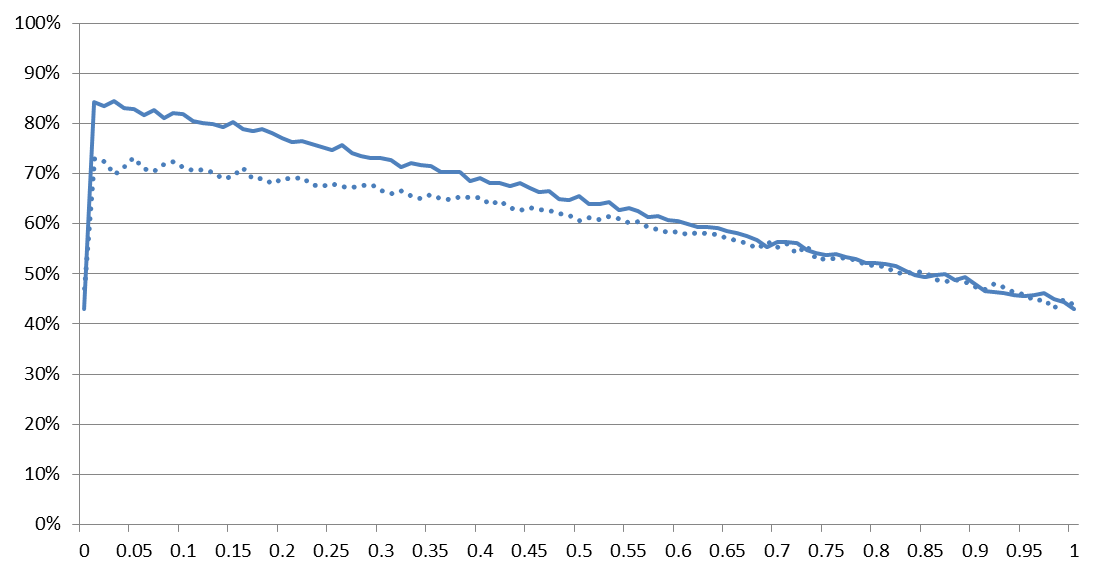
\includegraphics[width=0.49\linewidth]{TicTacToe_Normal_Vs_Symmetric_Equality_1280k.png} \label{ttt-n-vs-se-1280k}}

    \caption{Graphs of the percent of 10,000 testing episodes of Tic-Tac-Toe won by the MC agent versus the value of epsilon used, for different numbers of training epsiodes. In each graph, the x-axis shows the value of epsilon, the y-axis shows the percentage of testing episodes won, the dotted line shows the agent's performance in normal Tic-Tac-Toe, and the solid line shows the agent's performance in SE Tic-Tac-Toe.}
    \label{fig:tictactoe-normal-vs-symmetric-equality-epsilon}
\end{figure}

In all eight experiments, the SE implementation outperformed the normal implementation by roughly 10\%. Upon closer inspection, the normal implementation's best winning rate is around 60\% after the agent was trained for only 10,000 episodes (Figure \ref{ttt-n-vs-se-10k}) and this increases to around 70\% after 1,280,000 training episodes (Figure \ref{ttt-n-vs-se-1280k}). On the other hand, the SE implementation already reaches a winning rate of around 80\% after only 10,000 episodes (Figure \ref{ttt-n-vs-se-10k}) and this only improves by a few percentage points after 1,280,000 training episodes (Figure \ref{ttt-n-vs-se-1280k}).

This suggests that the SE implementation causes the MC agent's policy to converge much faster. To test this, we run performance experiments on both implementations for several values of epsilon and compare the results in Figure \ref{fig:tictactoe-normal-vs-symmetric-equality-performance}.

\begin{figure}
    \centering

    \subfigure[$\varepsilon$ = 0.01]{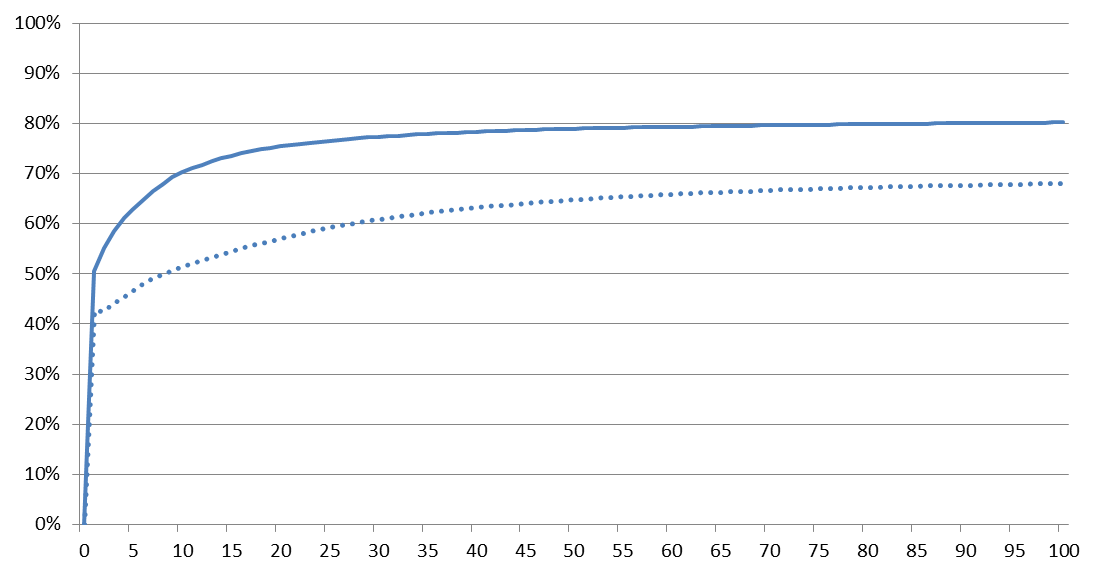
\includegraphics[width=0.49\linewidth]{TicTacToe_Normal_Vs_Symmetric_Equality_001.png} \label{ttt-n-vs-se-0-01}}
    \subfigure[$\varepsilon$ = 0.02]{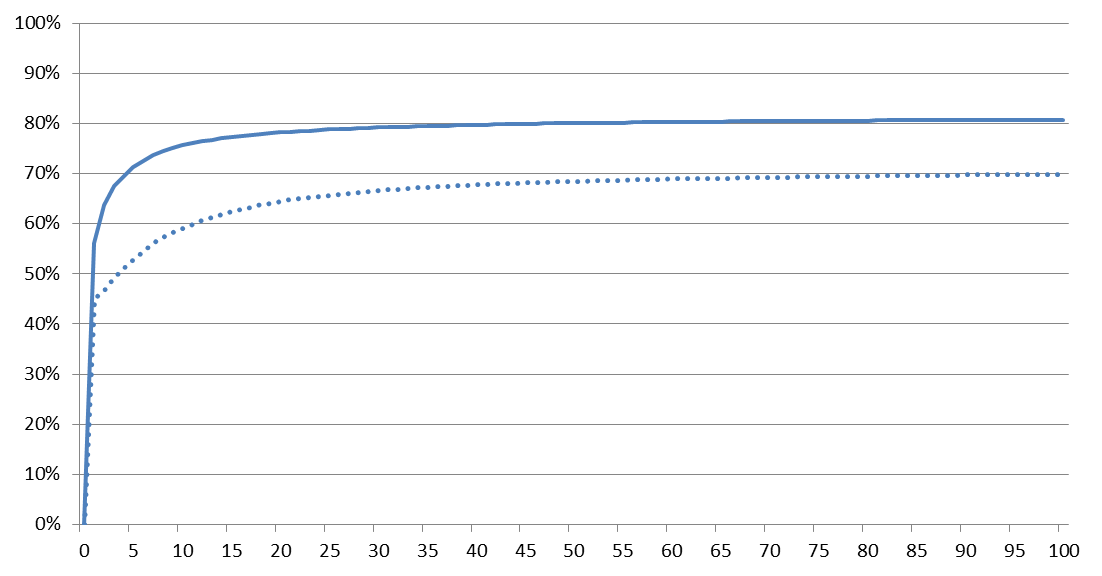
\includegraphics[width=0.49\linewidth]{TicTacToe_Normal_Vs_Symmetric_Equality_002.png} \label{ttt-n-vs-se-0-02}}
    \subfigure[$\varepsilon$ = 0.04]{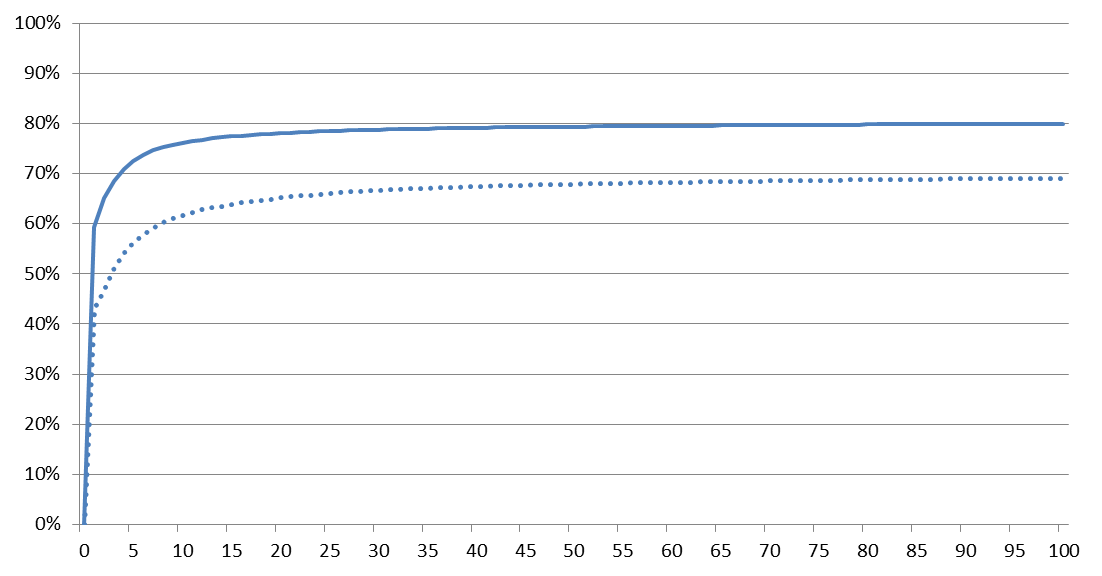
\includegraphics[width=0.49\linewidth]{TicTacToe_Normal_Vs_Symmetric_Equality_004.png}}
    \subfigure[$\varepsilon$ = 0.08]{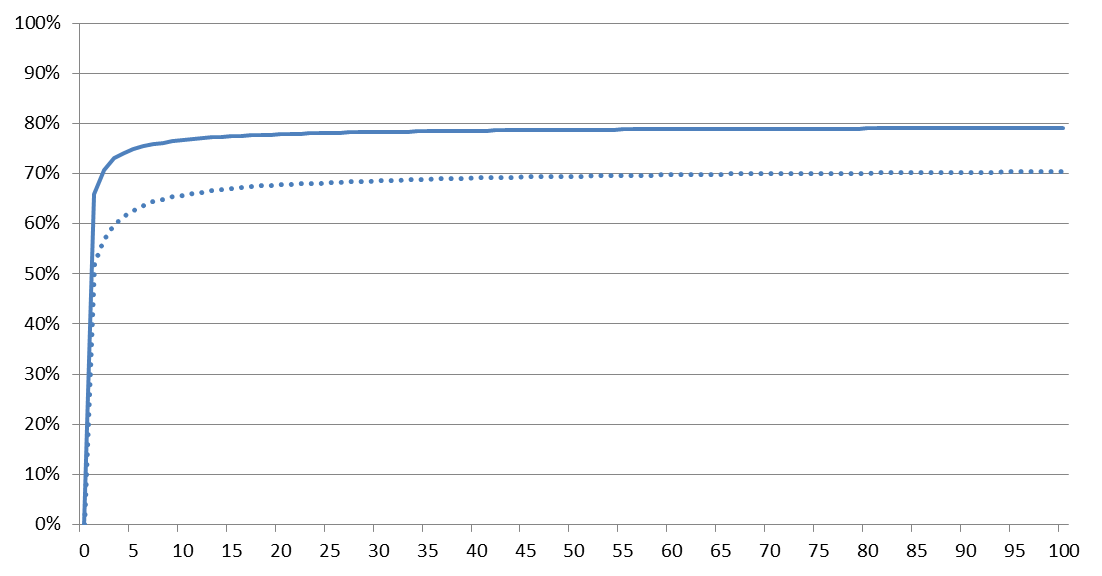
\includegraphics[width=0.49\linewidth]{TicTacToe_Normal_Vs_Symmetric_Equality_008.png}}
    \subfigure[$\varepsilon$ = 0.16]{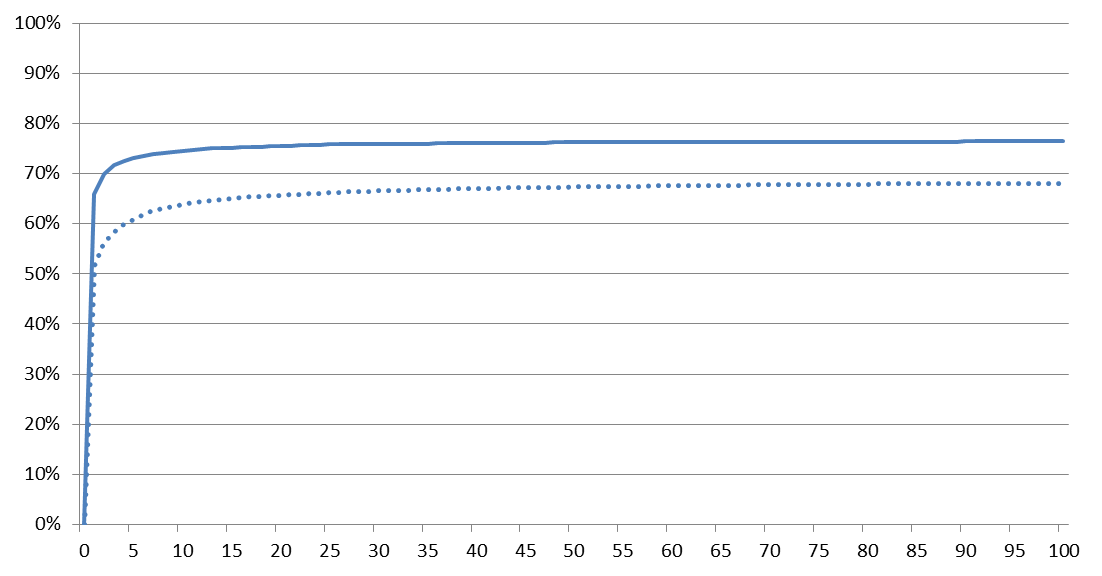
\includegraphics[width=0.49\linewidth]{TicTacToe_Normal_Vs_Symmetric_Equality_016.png}}
    \subfigure[$\varepsilon$ = 0.32]{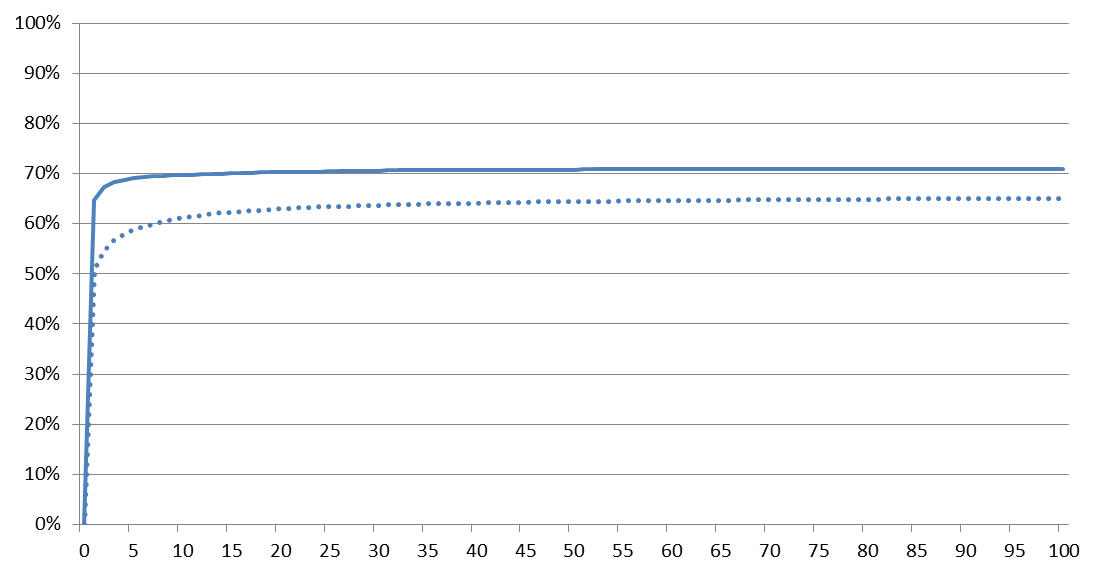
\includegraphics[width=0.49\linewidth]{TicTacToe_Normal_Vs_Symmetric_Equality_032.png}}
    \subfigure[$\varepsilon$ = 0.64]{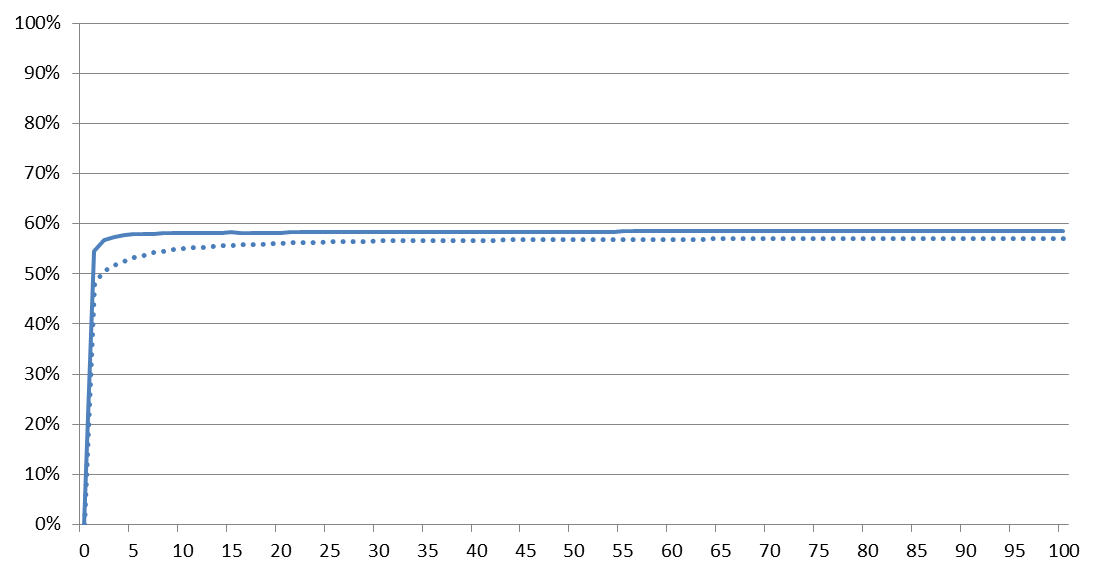
\includegraphics[width=0.49\linewidth]{TicTacToe_Normal_Vs_Symmetric_Equality_064.png}}

    \caption{Graphs of the MC agent's winning rate for increasing numbers of training episodes of normal Tic-Tac-Toe and of SE Tic-Tac-Toe. In each graph, the x-axis shows the number of training episodes ($10^4$), the y-axis shows the percentage of episodes won, the dotted line shows the agent's performance in normal Tic-Tac-Toe, and the solid line shows the agent's performance in SE Tic-Tac-Toe.}
    \label{fig:tictactoe-normal-vs-symmetric-equality-performance}
\end{figure}

The results are very interesting because the two curves are almost perfectly parallel in most of the seven experiments, particularly for the larger values of epsilon. In the first few experiments where epsilon is small, the normal implementation, which does not break symmetries, takes quite a bit longer to converge. This is particularly clear in Figures \ref{ttt-n-vs-se-0-01} and \ref{ttt-n-vs-se-0-02} because there is no visible ``elbow'' in the curve and the winning rate increases more gradually. This makes sense because when epsilon is small, more training episodes are needed in order for the agent to encounter more of the good/optimal state-action pairs. This effect is more subdued for the SE implementation because knowledge from symmetrical states is merged together, which has the same effect as playing more episodes.

All in all, it is quite clear that breaking symmetries in RL tasks can be hugely beneficial in terms of the agent's success rate (not to mention the reduced size of the state-value function). In the case of Tic-Tac-Toe, this can lead to a winning rate that is up to 10\% larger and for games or tasks with more axes of symmetry, it is reasonable to expect this figure to be even larger.


%-----------------------
\chapter{Discussion \& Future Work}

This chapter discusses a number of discrete ideas considered or investigated in this project, how some of these ideas have been studied, and what further work can be conducted.


\section{Using RL to Learn Epsilon}

A concept that was experimented with as part of this project was using a MC agent to learn the best value of epsilon to use for a certain game (Tic-Tac-Toe was arbitrarily chosen) and number of training episodes. The hope was that instead of making a human run the epsilon and convergence experiments described in Section \ref{sec:experiment-types} in order to manually determine an appropriate value of epsilon, a MC agent itself could learn such a value on its own. This can be thought of as ``meta-RL'' since RL is used to train a MC agent to choose epsilon parameters and then its findings (i.e. policy) are in turn used to initialise some other MC agent that is playing a game like Tic-Tac-Toe.

Since the \emph{MonteCarloAgent} class knows how to play games, this task was formulated as a game, with the usual classes that implement the \emph{Game}, \emph{State}, and \emph{Action} interfaces. The game was called ``Find Epsilon'', it was a one-player game, and each episode ended after the player chose one action. The state space consisted of a single state that contained no information and the actions available from that state were all possible values of epsilon from 0.0 to 1.0 inclusive (at some regular interval, such as 0.01). The return the agent received for choosing an action (i.e. value of epsilon, call it $x$) was the number of episodes a MC agent initialised with $\varepsilon = x$ won when playing Tic-Tac-Toe 100,000 times against an agent that plays randomly.

This seemed like a reasonable setup because the returns accurately reflected how well the agent was performing. However, when a MC agent was trained to play this game, it became clear that this was a highly inefficient way of finding good epsilon values. Since the game consisted of only one action, it would have been much more efficient to iterate through all possible epsilon values from 0.0 to 1.0 and for each one initialise a MC agent with that value and make it play Tic-Tac-Toe 100,000 times against an agent that plays randomly. For an epsilon precision of 0.01, this would mean that sessions of 100,000 Tic-Tac-Toe episodes would have to be played 101 times (one session per epsilon value) and then it would be clear which epsilon value resulted in the highest winning rate. In fact, this is precisely what the epsilon experiments described in Section \ref{sec:experiment-types} do. On the other hand, when the task is formulated as a Find Epsilon game, it takes much more than 101 sessions of 100,000 episodes before all values of epsilon are tried. The MC agent's policy is only useful if the agent has tried all possible epsilon values and so a lot of time and computational power is wasted while waiting for the agent to eventually try all values. Thus, this idea was abandoned and epsilon experiments were adopted instead.

The idea of using RL to learn good values for meta-parameters is not new -- in fact, a variety of research has been conducted on the topic of finding the right balance between exploration and exploitation in RL by finding good meta-parameters \cite{meta-optimization} \cite{meta-param-evolution} \cite{exploration-exploitation-meta-param} \cite{meta-learning-rl}. As a result, a number of algorithms have been developed in order to tailor meta-parameters that control this balance to the task at hand, including some based on genetic algorithms \cite{meta-param-evolution} for instance.

In particular, one paper \cite{meta-learning-rl} studied use of the soft-max function to compute the probability of taking an action. The formula for this probability function involves a meta-parameter $\beta$ called the ``inverse temperature'' that controls the exploration-exploitation tradeoff, just like $\varepsilon$ in the MC algorithm. A low value of $\beta$ corresponds to high exploration and a high value corresponds to high exploitation. The paper found that the best results were produced when $\beta$ \emph{dynamically adjusted} during a training session. It was found that even if $\beta$ was given a high value initially, it would start by decreasing to enable large exploration and then as the number of training episodes increased and its learning progressed, $\beta$ would start increasing to minimise exploration.

This finding makes a lot of sense and corresponds exactly to the conclusions drawn at the end of Section \ref{sec:convergence-results}. Since in this project $\varepsilon$ was fixed throughout training/testing sessions, the conclusion drawn from epsilon and convergence experiments was that a large value of epsilon (which corresponds to high exploration) should be used when relatively few training episodes can be run and a small value should be used when relatively many can be run. Combining these two ideas together, for any number of training episodes, epsilon should ideally start off large and then start decreasing for the best possible performance.

Thus, it would be very interesting to implement some of the algorithms developed to regulate the exploration-exploitation balance and combine them with the MC algorithm studied in this project. Most of the papers on this topic study algorithms that ``bootstrap'' (i.e. update the values of states using estimates of the values of subsequent states \cite{rl-book}) such as Temporal Difference learning. Studying how an algorithm that allows $\varepsilon$ to dynamically adapt during training works with a learning technique that does not bootstrap might therefore produce novel results.


\section{Optimality of Learned Policies}
\label{sec:policy-optimality}

Section \ref{sec:experiment-types} is intentionally vague about what a policy might converge to and whether it converges to some optimal policy. It is important to note two important results before continuing:

\begin{itemize}
    \item The $\varepsilon$-soft on-policy MC control algorithm studied in this project has \emph{not} yet been proven to converge to an optimal policy \cite{open-rl-questions}. This means that even if the curve produced by a convergence experiment clearly flattens, it may very well be that the agent has found some local maximum.
    \item There is a stationary deterministic optimal policy for every Markov Decision Process (MDP) \cite{mdp-convergence}, which means that, at the very least, there \emph{is} some optimal policy for all three games studied in this project. However, there is no way of knowing for sure whether this is the policy that the MC agent converges to.
\end{itemize}

Having mentioned these two results, it is clear that the results of the convergence experiments described in Section \ref{sec:convergence-results} are not very conclusive because all they show is that the MC agent converges to \emph{some} policy after sufficient training episodes. Nevertheless, this is still a useful result because a reasonably quick convergence to a good policy is often preferable to a slow convergence to the optimal policy \cite{rl-a-survey}.


\section{Alternative Tic-Tac-Toe Implementation That Breaks Symmetry}

Another way of eliminating symmetry in Tic-Tac-Toe was also considered: limiting the actions available from each state such that no two actions result in symmetrical states. An interesting result of this idea is that it would slightly alter the way the game is played. Suppose a random agent is asked to select a move from the game's initial state (i.e. empty grid). In the Normal implementation, there are nine possible actions: putting an \textbf{X} token in one of the nine grid cells. In this ``Limited Actions'' version, there are only three possible actions: putting an \textbf{X} token in a corner, in the middle of the grid, and in the middle of one of the sides. To give a specific example of how this would change the game, notice that the probability of the agent choosing the action that involves placing their token in the middle of the grid is $\frac{1}{9}$ in the Normal implementation and $\frac{1}{3}$ in the Limited Actions version. Thus, the agent will end up choosing this action three times as frequently in the latter version.

In the limit of infinitely many games, however, the MC agent would encounter all states and choose all possible moves an equal number of times, thus computing an accurate expected return for each action. It would be interesting to compare the performance of such a Limited Actions implementation with the Symmetric Equality implementation. Both should perform equally well on any game given enough training, but it is possible that they might improve at different rates.


\section{More... to be discussed}


%-----------------------
\chapter{Conclusion}




\section{Personal Reflections}

This has been a really great learning experience, not only in terms of discovering the field of reinforcement learning and its applications, but also in terms of gaining experience with building up a large, complex programming project from scratch using a variety of technical tools.

When I was in high school, I designed and implemented the classic board game Nine Men’s Morris where a user plays against an algorithm I wrote. My plan for the project was to ask my friends and family to play my game and to store the moves made in each game so that I could build up a database of sequences of moves and outcomes of the game. I hoped to somehow compute which moves were the best and get my algorithm to learn which moves made winning the most likely. Little did I know, I wanted to invent RL from scratch – unaware of its existence or of the amount of research in the field. Several years later, I am delighted to have had the chance to work on a similar project, but this time on a deeper level using well-known computational algorithms. [\emph{I don't know if this paragraph should stay in my final version...}]

When I started working on this project, I decided to treat it as an opportunity to develop many skills that are critical for a career in software engineering:

\begin{itemize}
	\item Writing clean, maintainable, well-documented code
	\item Designing and implementing tests for my code
	\item Using a build tool to manage dependencies between packages in my project as well as with external libraries
	\item Using version control effectively
\end{itemize}

I tested the methods in my API using a unit-testing framework for Java called JUnit. I also used a testing framework for Java called Mockito – this allowed me to verify the behaviour of objects with external dependencies by creating “mock objects” for theses dependencies, which mimic real objects but do so in a particular way that I can specify.

In order to save my experiment results in a format that would facilitate the creation of graphs, I used opencsv, a CSV parser library for Java.

To manage my project’s dependencies, I used a build tool developed by Google called Bazel and I used Git for version control.

Overall, I really enjoyed learning about RL algorithms and exploring their applications and success rates, all while developing strong programming skills that will help me throughout my career.


%--------------------------------
\chapter{Acknowledgements}



%--------------------------------
\bibliography{mybib}{}
\bibliographystyle{plain}

\end{document}
